\documentclass{tudelft-report}

%% Set up the bibliography
\usepackage{biblatex}
\addbibresource{references.bib}

%% Additional packages and commands
\usepackage{parskip}
\setlist{itemsep=-2pt} % Reducing white space in lists slightly
\renewcommand{\deg}{\si{\degree}\xspace} % Use \deg easily, everywhere

%% ----------------------------------------------------------------------
%%    Begin of document + Frontmatter (Roman page numbering)
%% ----------------------------------------------------------------------

\begin{document}

\frontmatter

%% Define the main parameters
\title{Design and analysis of a SEMSANS instrument for a cold source}
%\subtitle{A Catchy Optional Subtitle \\ that Grabs the Attention}
\author{T.\ B.\ van der Woude}

%\subject{AB1234: Optional Course Name} % Cover only
\affiliation{Delft University of Technology} % Cover only
\coverimage{figures/cover2.jpg} % Aspect ratio of 2:3 (portrait) recommended
\definecolor{title}{HTML}{4884d6} % Color for cover title

\makecover

% \input{frontmatter/title-report}
\begin{titlepage}

\begin{center}

%% Print the title
{\makeatletter
\largetitlestyle\fontsize{45}{45}\selectfont\@title
\makeatother}

%% Print the subtitle
{\makeatletter
\ifdefvoid{\@subtitle}{}{\bigskip\titlestyle\fontsize{20}{20}\selectfont\@subtitle}
\makeatother}

\bigskip
\bigskip

by

\bigskip
\bigskip

%% Print the name of the author
{\makeatletter
\largetitlestyle\fontsize{25}{25}\selectfont\@author
\makeatother}

\bigskip
\bigskip

to obtain the degree of Bachelor of Science
%ter verkrijging van de graad van Master of Science

at the Delft University of Technology,
%aan de Technische Universiteit Delft,

to be defended publicly on Monday June 4, 2024 at 10:00 AM.
%in het openbaar de verdedigen op maandag 1 januari om 10:00 uur.

\vfill

\begin{tabular}{lll}
    Student number: & 4945727 \\
    Project duration: & \multicolumn{2}{l}{April 22, 2024 -- June 4, 2024} \\
    Thesis committee: & Prof.\ dr.\ W.\ G.\ Bouwman & TU Delft, supervisor \\
        & Dr.\ Ing.\ J.\ Plomp, & TU Delft
\end{tabular}

%% Only include the following 3 lines if confidentiality is applicable.
\bigskip
\bigskip
%\emph{This thesis is confidential and cannot be made public until December 31, 2024.}
%\emph{Op dit verslag is geheimhouding van toepassing tot en met 31 december 2024.}

\bigskip
\bigskip
\begin{tabular}{p{15mm}p{10cm}}
			Cover: & A ray-traced 3D plot of simulated detector counts for a dilute sample solution of solid spheres with $R = \SI{300}{\nano\meter}$ with a modulated beam. On the axes are the detector $y$-coordinate and source wavelength $\lambda$. The source is monochromatic and $\lambda$ varies from $\SI{2}{\angstrom}$ to $\SI{12}{\angstrom}$.\\
    % Feel free to remove the following attribution, it is not required - still appreciated :-)
    % Style: & TU Delft Report Style, with modifications by Daan Zwaneveld
\end{tabular}

\bigskip
\bigskip
An electronic version of this thesis is available at \url{http://repository.tudelft.nl/}.

\end{center}

%% Insert the TU Delft logo at the bottom of the page
\begin{tikzpicture}[remember picture, overlay]
    \node[above=10mm] at (current page.south) {%
        \includegraphics{figures/logo-black}
    };
\end{tikzpicture}

\end{titlepage}

% \input{frontmatter/preface}
\chapter*{Summary}
\addcontentsline{toc}{chapter}{Summary}

\emph{A summary...}


\tableofcontents
%\listoffigures
%\listoftables

% \input{frontmatter/nomenclature}

%% ----------------------------------------------------------------------
%%    Mainmatter (Arabic page numbering)
%% ----------------------------------------------------------------------

\mainmatter
\chapter{Introduction}
\label{chapter:introduction}
\label{c1:introduction}
In many industries, there is the need to analyse the structure of materials at length scales ranging from nanometres to micrometers. To do this, different methods exist such as scattering techniques, microscopy and analysis based on macroscopic properties. What is unique about scattering techniques however is that they can probe the bulk of the sample at these length scales \cite{bouwman2021}.

% I need to add a better bridge between these two sections, they are both good but lack coupling.

\section{Small-angle scattering}
\label{c1.1}
Different scattering techniques exist based on X-rays and neutrons. Generally speaking, because these are reciprocal space methods, larger length-scales correspond to smaller scattering angles and vice versa. This is the motivation behind small-angle scattering methods like Small Angle X-ray Scattering (SAXS) and Small Angle Neutron Scattering (SANS) which are used to analyse materials at length scales from $\SI{1}{\nano\meter}$ to a few $\SI{100}{\nano\meter}$, which are significantly larger than for instance crystal lattice constants of a few $\unit{\angstrom}$ that can be determined using techniques like X-ray diffraction. Past the upper limit of a few $\SI{100}{\nano\meter}$ such small-angle techniques become infeasible for realistic beam sizes and samples, as the deflection of particles in a beam is too slight to learn something about the sample.

For neutrons, spin polarization can be used to label trajectories across the beam, a technique called neutron spin echo \cite{mezei1972}. This principle has been applied in the SANS-derivative techniques SESANS \cite{rekveldt1996} and SEMSANS \cite{bouwman2009}\cite{bouwman2011} to make smaller angles and correspondingly the larger length scales up to about $\SI{10}{\micro\meter}$ accessible using polarized neutrons. Formulated differently, these techniques can be seen to measure a type of real-space density correlation function $G(\delta)$ \cite{krouglov2003}\cite{andersson2008} as will also be discussed in Chapter \ref{c2:theory}.

\section{SEMSANS at the Reactor Institute Delft}
\label{c1.2}

SEMSANS instruments have previously been realized at the Hoger Onderwijs Reactor (HOR) at the Reactor Institute Delft (RID) using a thermal neutron source. As part of the OYSTER project (Optimized Yield for Science, Technology, and Education of Radiation), a cold neutron source operating at $T=\SI{20}{\kelvin}$ has been installed and additional improvements have been made to achieve an expected hundredfold improvement in measurement quality or time.

In this report, the possibility for realizing a SEMSANS instrument at the new cold source at HOR will be explored through a combination of mathematical analysis, constrained optimization and Monte Carlo simulations using raytracing software package McStas \cite{willendrup2020}. An existing McStas simulation model \cite{bouwman2021b} is taken as a starting point and extended to include various design options such as precession devices different from foil flippers. 
The goal is to bridge the gap between accessible length ranges of SANS and SEMSANS \cite{bouwman2021} and see if it is possible to access characteristic lengths from $\SI{10}{\nano\meter}$ to $\SI{5}{\micro\meter}$ in a single instrument by exploiting the advantage of greater wavelengths. This as an alternative to combining SANS and SEMSANS devices into one as has been proposed before \cite{bouwman2011}\cite{kusmin2017}. An application in the food industry that would benefit from such an instrument is the study of colloids such as casein micelles in (fat free) milk and derivatives like yoghurt and curd. The characteristic length scales of all of these would be accessible at an instrument with this target range, facilitating a better understanding of processes like milk turning into yoghurt. 
\chapter{Theory}
\label{chapter:theory}
\label{c2:theory}
In this chapter, a review is given of relevant theory related to SEMSANS and the interpretation of measurements. First, the basic principles of SEMSANS as a neutron spin echo technique are explained and the way the beam is modulated is derived. Next, the interaction of samples with the modulated beam is discussed and the concept of spin-echo length $\delta$ and introduced as a way of characterizing a sample by considering its SESANS correlation function $G(\delta)$. Lastly, a reference sample that will be used throughout this work is introduced and characterized by its $G(\delta)$ and form factor $P(Q)$. 

% I like 'Beam modulation through Larmor precession' as a phrase
\section{Polarized neutrons and Larmor precession}
\label{c2.1}
Neutrons are spin $s=\frac{1}{2}$ particles with a spin angular momentum vector $\vec{S}$, the direction of $\vec{S}$ being the spin polarization $\vec{P}$. When a neutron passes through a uniform $\vec{B}$-field, $\vec{P}$ will precess by a certain angle $\phi$ over time. The frequency at which this occurs is given by
$$\omega = \gamma |B_\perp|$$
with $B_\perp$ the magnetic field strength perpendicular to the plane $\vec{P}$ is in and $\gamma$ the neutron gyromagnetic ratio. In addition to spin, a neutron has a wavelength $\lambda$ corresponding to a speed $v = \frac{h}{m\lambda}$, $m$ being the neutron mass. This means that it will pass through a uniform (perpendicular) field $B$ of length $L$ in time $t = \frac{Lm\lambda}{h}$. From this it can be seen that the total precession will be 
\begin{equation}
	\phi = \frac{\gamma B L m\lambda}{h} = c\lambda B L \label{eq:larmor-prec}
\end{equation}
with $c = \frac{\gamma m}{h}$ being the Larmor constant \cite{bouwman2021b}.   
\section{Modulating a neutron beam using precession}
\label{c2.2}
Using the concepts of polarized neutrons and Larmor precession, the basic concept of a SEMSANS instrument can be described, deferring a detailed discussion of the source and monochromator for now. The instrument takes a neutron beamline as a source, meaning that with the choice of axes used in this research, neutrons can be assumed to move in the $z$-direction with a slight divergence in the $xy$-plane. A polarizer is used to polarize the beam in the $+x$ direction. Next, the beam passes through two precession devices  that give neutrons at wavelength $\lambda$ in the beam a $y$-dependent precession angle in the $xz$-plane due to an applied $B_y$-field %at distance $L_1, L_2$ from the detector
\begin{equation}
	\phi = 2\pi\alpha\lambda y \label{eq:precession-freq}
\end{equation}
with $\alpha$ being a constant specific to the used precession device that together with $\lambda$ determines the precession frequency. This precession can be thought of as $\vec{P}$ being rotated over a $y$-dependent angle $\phi$. Such a $y$-dependent $\phi$ is in practice created by using $B_y$-fields with interfaces at an angle $\theta_0$ with the beam axis $z$. Different precession devices exist which can create such fields as will be analysed and discussed in Section \ref{c3.3}.

Finally, the modulation is created by applying an analyser to the beam afterwards \cite{mezei1972}. This again polarizes the beam in either the $+x$ or the $-x$ direction depending on the analyzer setting. Assuming a perfectly monochromatic source with wavelength $\lambda = \lambda_0$, this creates an intensity modulation pattern on the position-sensitive detector at frequency $f_0 = \alpha\lambda_0$ of the form
\begin{equation}
	I_{b,s}(y) = I_{0, b,s} \pm A_{b,s}\cos(2\pi f_0y) \label{eq:mono-modulation}
\end{equation}
where $I_{b,s}, A_{b,s}$ are experimentally observed quantities in the base case of an empty instrument ($b$) and for an instrument with a sample ($s$) and the sign of the modulation depending on the $\pm x$ analyser setting \cite{parnell2023}. 
\section{Spin-echo length $\delta$ and measurement interpretation}
\label{c2.3}
When adding a sample to the instrument after the analyser at distance $L_s$ from the detector, a correlation length known as the spin-echo length $\delta$ is accessed \cite{bouwman2011}, given by 
\begin{equation}
	\delta = \lambda_0^2L_s\alpha \label{eq:delta}
\end{equation}
Assuming a measurement along the $y$-axis, the above can be derived from the wave-vector transfer $Q_y$ using the small-angle expression $Q_y = \frac{2\pi}{\lambda}\frac{y}{L_s}$. In this way, $\phi$ can be rewritten to $\phi = \delta Q_y$ with $\delta$ as given. It is the same spin-echo length as used in the analysis and interpretation of SESANS \cite{rekveldt1996}\cite{krouglov2003}\cite{andersson2008}. Whereas in SESANS a decrease in overall beam polarization is used, SEMSANS considers the reduction of intensity modulation amplitude or equivalently visibility upon adding a sample, which can be shown to be related to $\delta$ through the formula \cite{parnell2023}
\begin{equation}
	\frac{A_s(\delta)}{A_b(\delta)} = P(\delta) = e^{G(\delta) - \tau} \label{eq:sample-pol-reduction}
\end{equation}
with $\tau = \sigma t$ being the scattering power, which corresponds to the average number of scattering events for a neutron traversing the sample. $t$ is the sample thickness and $\sigma$ is the total scattering cross-section defined by 
\begin{equation}
	\sigma = \frac{1}{k_0^2}\int_{-\infty}^\infty\int_{-\infty}^\infty\dfrac{d\sigma(\vec{Q})}{d\Omega}dQ_xdQ_y  \label{eq:sigma-analytical}
\end{equation}
$G(\delta)$ is the SESANS correlation function given by
\begin{equation}
	G(\delta) = \frac{t}{k_0^2}\int_{-\infty}^\infty\int_{-\infty}^\infty\dfrac{d\sigma(\vec{Q})}{d\Omega}\cos(Q_y \delta)dQ_xdQ_y  \label{eq:G-analytical}
\end{equation}
This is the 1D expression for $G(\delta)$ matching the 1D detector that will be described in the next chapter. In words, $G(\delta)$ is a cosine transform of $d\sigma(\vec{Q})/d\Omega$ \cite{li2019} along the $y$-axis with regular integration over the $x$-axis. Although formally the integration range is infinite, for practical samples the relevant $Q$-range where $d\sigma(\vec{Q})/d\Omega$ is significantly greater than zero will be limited as will be discussed for a particular sample in the next section. This makes it possible to approximate this cosine transform integral over the finite $Q$-range accessible at a detector, relying on the principle that for large enough samples most neutrons will reach the detector \cite{rekveldt1996}. This framework has been extended to 2D using a two-dimensional cosine transform, making it possible to analyse anisotropic samples using a 2D modulated beam \cite{parnell2023}.
For isotropic samples, radial integration is possible without loss of information and $G(\delta)$ can be stated using a Hankel transform instead of a cosine transform \cite{andersson2008}.

\section{Mono-disperse reference sample and its $G(\delta)$}
\label{c2.4}
Expressions for $\tau$ and $G(\delta)$ exist and can be derived for many different sample geometries \cite{andersson2008}. In the context of analysing colloidal systems, a simple commonly used model is a dilute mono-disperse solution of solid spheres \cite{tromp2007}. Although poly-disperse models such as log-normal distributions of spheres appear to better match real samples \cite{heijkamp2011}, a mono-disperse sample is used as a reference in this work as it is also implemented in McStas in the form of the \texttt{SANS\_spheres2} component (see \cite{parnell2024} for a validation of this sample in the context of SESANS) in addition to being a simpler model for samples of various characteristic lengths. Such a mono-disperse sample is characterized by sphere radius $R$, scattering length density contrast $\Delta\rho$, volume fraction $\phi$ and sample thickness $t$. The scattering power $\tau$ for such a sample is given by
\begin{equation}
	\tau = \frac{3}{2}\phi (1 - \phi) (\Delta\rho)^2\lambda_0^2tR \label{eq:sample-tau}
\end{equation}
Using $\xi = \frac{\delta}{R}$, it can be derived that for $0\leq \xi \leq 2$, $G(\delta) = \tau G_0(\delta)$ with 
\begin{equation}
	G_0(\delta) = \left[1 - \left(\frac{\xi}{2}\right)^2\right]^{1/2}\left(1 + \frac{1}{8}\xi^2\right) + \frac{1}{2}\xi^2\left[1 - \left(\frac{\xi}{4}\right)^2\right]\ln \left[\frac{\xi}{2 + (4 - \xi^2)^{1/2}}\right] \label{eq:sample-G0}
\end{equation}
$G_0(\delta)$ is the normalized correlation function with key property $G_0(0) = 1$ as opposed to $G(0) = \tau$. Outside of this range, $G_0(\xi) = 0$ \cite{krouglov2003}. Figure \ref{fig:analytical-G0} shows $G_0(\delta)$ for different values of $R$. 

\begin{figure}
	\centering
	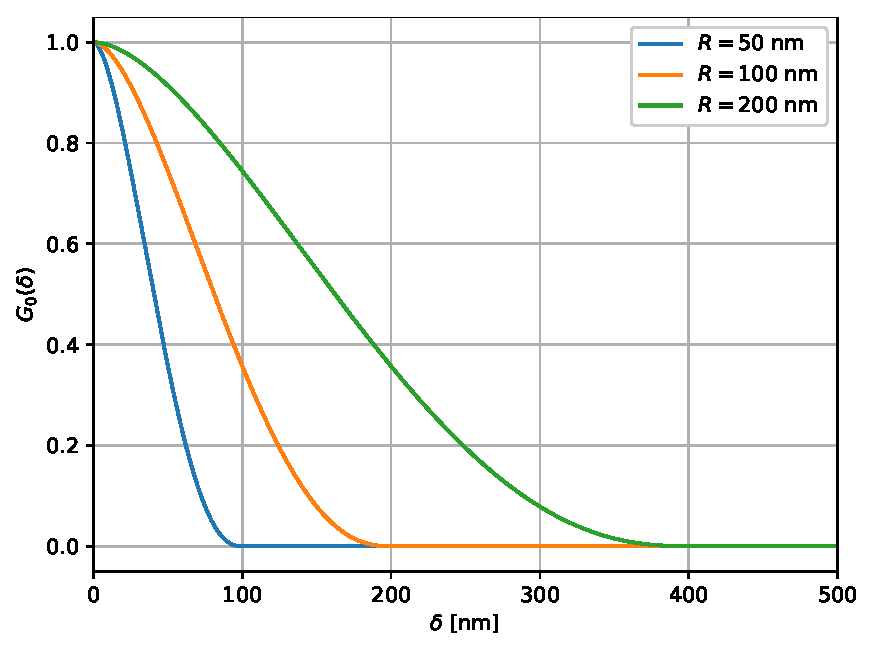
\includegraphics[width=0.5\linewidth]{analytical-G0}
	\caption{Normalized SESANS correlation function $G_0(\delta)$ curves for three dilute mono-disperse solid sphere samples with different radii $R$. The corresponding analytical expression is given by Equation \eqref{eq:sample-G0}.}
	\label{fig:analytical-G0}
\end{figure}

\subsection{Solid sphere form factor and $Q$-range}
Formulated in terms of $Q$ as in regular SANS rather than $\delta$, the relevant $Q$-range of a dilute mono-disperse sample of spheres with radius $R$ can be seen to be largely determined by its form factor $P(Q)$ as $d\sigma(\vec{Q})d\Omega\propto P(Q)$, which is \cite{rekveldt1996}
\begin{equation}
	P(Q) = \left(3\frac{\sin(QR) - QR\cos(QR)}{\left(QR\right)^3}\right)^2\label{eq:sample-form-factor}
\end{equation}
This is a rapidly decaying oscillation with significant values in the range from $Q_{\text{min}} = 0.1/R$ up to $Q_{\text{max}} = 10/R$, meaning that in order to determine $G(\delta)$ accurately a detector should integrate over a proportional $Q$-range.  Figure \ref{fig:analytical-P} shows $P(Q)$ with these limits for $R = \SI{100}{\nano\meter}$.  

\begin{figure}
	\centering
	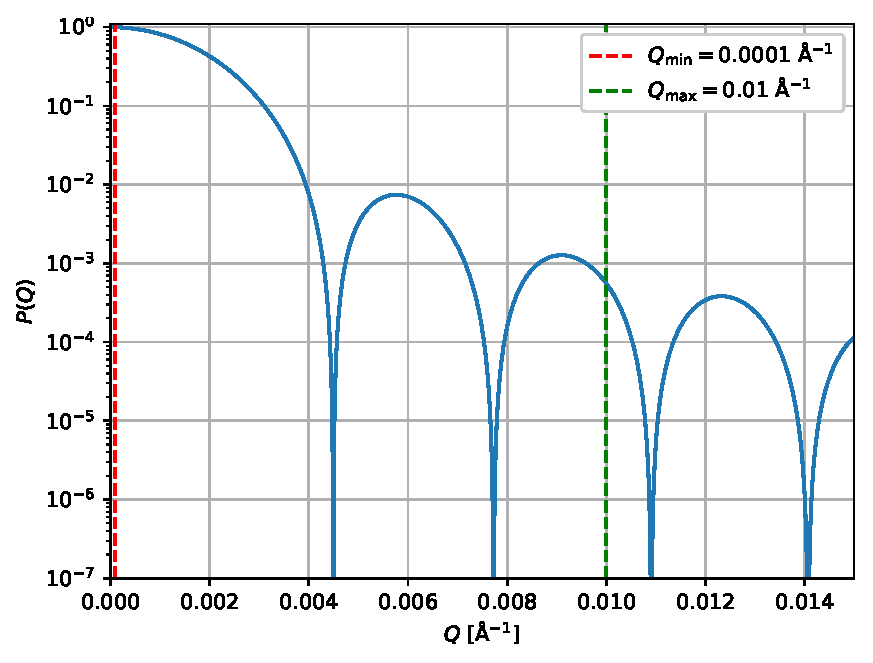
\includegraphics[width=0.5\linewidth]{analytical-P-log}
	\caption{Solid sphere form factor $P(Q)$ for $R = \SI{100}{\nano\meter}$ with $Q_{min}, Q_{max}$ as given by Equation \eqref{eq:sample-form-factor}. It can be seen that for $Q > Q_{max}$, $P(Q) < 10^{-3}$ with its oscillation peaks decreasing in amplitude.}
	\label{fig:analytical-P}
\end{figure}
\chapter{Instrument analysis for a cold source}
\label{chapter:introduction}
\label{c3}
\begin{figure}[hbtp]
	\centering
	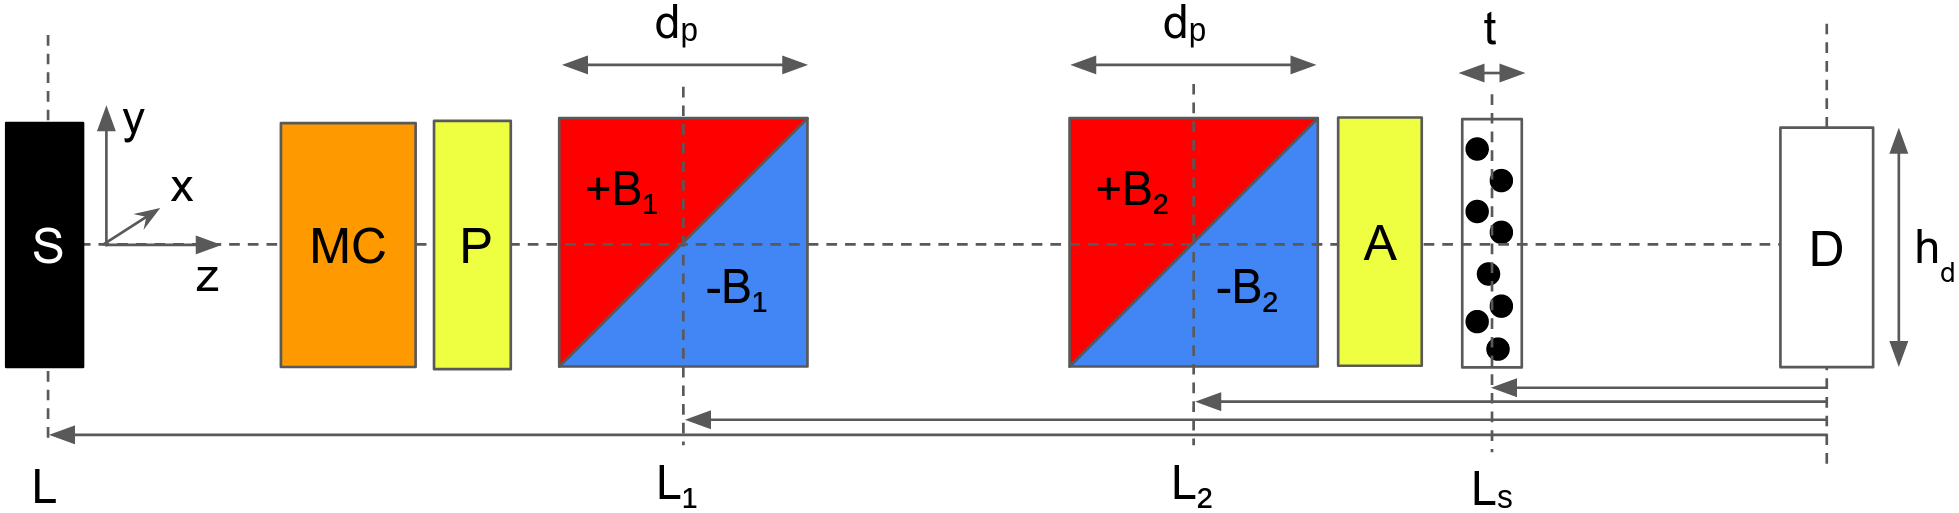
\includegraphics[width=\linewidth]{instrument-configuration}
	\caption{A schematic of the SEMSANS instrument configuration considered in this chapter. Lengths and dimensions are not to scale. Neutrons are emitted from the source (S) after which they pass through a monochromator (MC) and are polarized in the $+x$ direction by a polarizer (P). The polarized neutrons travel through two precession devices (shown are Wollaston prisms as discussed in Section \ref{c3.3}) at distances $L_1, L_2$ from the detector. These devices have field strength $\pm B_1$ and $\pm B_2$ in different field regions to create a $y$-dependence in the precession angle as discussed in Section \ref{c2.2} and have depth $d_p$. Next, the beam passes through an analyzer (A) which can be in the $+x$ or $-x$ setting, creating a modulated intensity pattern. This modulated beam scatters of the sample with thickness $t$ at distance $L_s$ from the detector, arriving at the detector (D) with height $h_d$. The sample can be removed to measure the unscattered modulation pattern, making it possible to compute the decrease in modulation visibility related to $G(\delta)$ as per Equation \eqref{eq:sample-pol-reduction}.}
	\label{fig:instrument-config}
\end{figure}

In this chapter, the SEMSANS instrument model used in this work is introduced and analyzed. The cold neutron source and the applicable monochromators for different $\lambda_0$ ranges will be described and three different precession device options and their properties will be discussed. Additionally, the effect of a spread in wavelength $\lambda$ on the observed modulation pattern and what is effectively measured will be considered. This is to account for the greater wavelength spread $\Delta\lambda/\lambda_0$ encountered when using a velocity selector as a monochromator, which is necessary at higher $\lambda_0$ operating points accessible at a cold source. In the last section, a list of instrument design variants considered in this research is introduced. These will be analyzed and simulated in Chapter \ref{c4:constraints} and Chapter \ref{c6:monte-carlo} respectively. 

\section{Instrument configuration}
\label{c3.1}
The general SEMSANS instrument model considered in this work is illustrated in Figure \ref{fig:instrument-config}. It is derivative of an existing study simulating a SEMSANS instrument using ferromagnetic foil-flippers and the corresponding McStas instrument \texttt{SEMSANS\_Delft} \cite{bouwman2021b}. Neutrons enter the instrument from a source, after which they pass through a monochromator set to select neutrons with a wavelength around $\lambda_0$, with  $\Delta\lambda/\lambda_0$ depending on the choice of monochromator as described below. Next, they pass through a polarizer and two precession devices at locations $L_1, L_2$ respectively. As described in Chapter \ref{c2:theory}, a modulated neutron intensity pattern appears after the analyzer, which scatters of the sample at distance $L_s$ from the position-sensitive detector at the end, causing different degrees of loss of visibility of the modulation pattern depending on the sample structure as discussed in Section \ref{c2.3}. 

\section{Source beam characteristics and monochromators}
\label{c3.2}
The cold source is assumed to have a spectrum corresponding to a Maxwell-Boltzmann distribution at $T = \SI{20}{\kelvin}$ given by 
\begin{equation}
	f_\lambda(\lambda) = \sqrt{\frac{2}{\pi}}\left(\frac{1}{mk_BT}\right)^{\frac{3}{2}}\frac{h^3}{\lambda^4}e^{-\frac{h^2}{2k_BTm\lambda^2}} \label{eq:cold-source-spectrum}
\end{equation}
This distribution is shown in Figure \ref{fig:source-spectrum}, with the thermal distribution at $T= \SI{290}{\kelvin}$ also shown for reference. For simplicity, a uniform rectangular beam of size $10\times10~\unit{\milli\meter}$ is used to model the beam and it is focussed on the middle $10\times10~\unit{\milli\meter}$ of the detector. Each neutron originating from point $(b_x,b_y)$ in the beam will be aimed at a uniformly sampled random point $(d_x, d_y)$ on the detector, so assuming a distance $L = \SI{5}{\meter}$ from source to detector the divergence will be at most $\psi_0 = \SI{2}{\milli\radian}$ along the $x$ or $y$ axis and about $\psi_0 = \SI{2.8}{\milli\radian}$ in total. This model corresponds to a rectangular setting of the \texttt{Source\_simple} McStas source component which will be used in Monte Carlo simulations in Chapter \ref{c6:monte-carlo}.  

% The peak for $T= \SI{20}{\kelvin}$ corresponds to $E = k_bT = \SI{1.7}{\milli\electronvolt}$ as opposed to $E = \SI{25.0}{\milli\electronvolt}$ for thermal neutrons. 
\subsection{Monochromators}
A monochromator is used to select a narrow band of wavelengths around a central wavelength $\lambda_0$. In a practical instrument, a pyrolytic graphite (PG) crystal monochromator can be used to do this up to roughly $\lambda_0 \approx \SI{4.4}{\angstrom}$. For greater wavelengths, a velocity selector (VS) can be used to select neutrons traveling at the right velocity. This is a mechanical device rotating at a great speed, and a lower practical limit of $\lambda_0 \approx \SI{7}{\angstrom}$ is used as lower $\lambda_0$ would require a too great RPM. Both types of monochromators are characterized by $\Delta\lambda/\lambda_0$, the ratio of the full-width-half-maximum (FWHM) of wavelengths $\Delta\lambda$ passed through and $\lambda_0$. In PG crystals, this is a function of the mosaicity of the crystal \cite{shapiro1972} and for velocity selectors, it depends on the ratio of the angular aperture of slits and the pitch angle \cite{szewc2010}. This ratio is taken to be $\Delta\lambda/\lambda_0 = 0.01$ and $\Delta\lambda/\lambda_0 = 0.1$ for the PG monochromator and velocity selector respectively, roughly corresponding to the characteristics of components available for an eventual realization. The transfer of these monochromators is taken to be a Gaussian centered at $\lambda_0$ with $\sigma = \frac{1}{2\sqrt{2\ln 2}}\Delta\lambda$, resulting in a selected $\lambda$-spectrum that can be approximated as Gaussian. This motivates the use of the following Gaussian distribution as a model spectrum after the monochromator in both analysis and simulations.
\begin{equation}
	f_\text{gauss}(\lambda) = \frac{1}{\sigma\sqrt{2\pi}} e^{-\frac{1}{2}(\frac{\lambda - \lambda_0}{\sigma})^2} \label{eq:gauss-spectrum}
\end{equation}
\begin{figure}
	\centering
	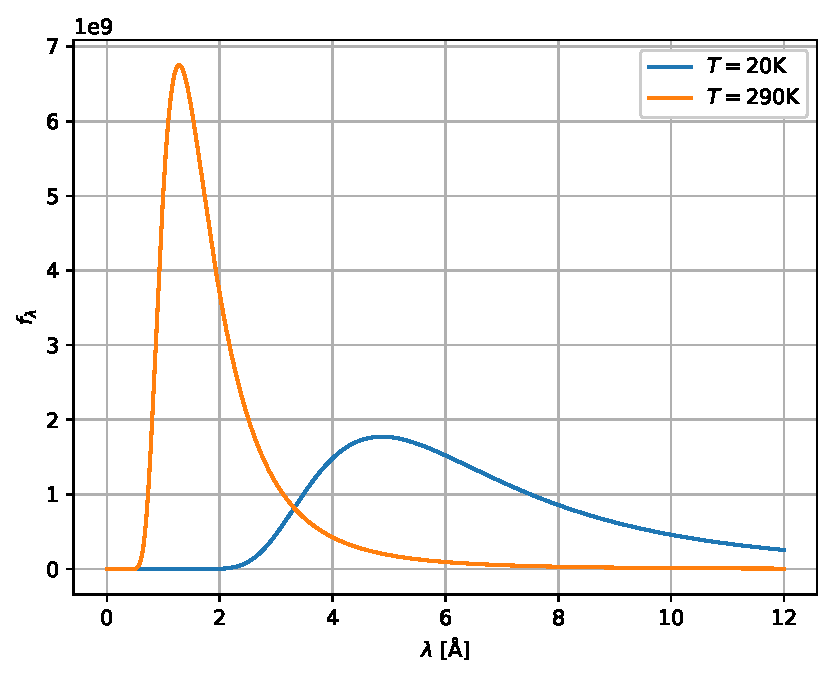
\includegraphics[width=0.5\linewidth]{source-spectrum}
	\caption{Probability density functions for Maxwell-Boltzmann neutron sources at $T = \SI{20}{\kelvin}$ and $T = \SI{290}{\kelvin}$, illustrating the spectral differences. }
	\label{fig:source-spectrum}
\end{figure}
\section{Precession device analysis}
\label{c3.3}
As discussed in Chapter \ref{c2:theory}, different precession devices can be derived that give a precession angle of the form of Equation \eqref{eq:precession-freq} resulting in modulation. The three main types existent in literature are isosceles triangles \cite{sales2015}, magnetic Wollaston prisms \cite{li2021} and ferromagnetic foil flippers \cite{bouwman2021b} and all three have previously been used in SEMSANS realizations and simulations. Their respective geometries are shown in Figure \ref{fig:precession-devices}. What they all have in common is that their effect is proportional to $\cot(\theta_0)$ and magnetic field strength $B$. Here, $\theta_0$ is the angle the magnetic field interfaces make with the $z$-axis in the $yz$ plane.
\subsection{Isosceles triangles}
In the case of an isosceles triangle as illustrated in Figure \ref{fig:precession-devices:iso}, the angle of the magnetic field interfaces with the $z$-axis can be seen to be $\theta_0 = \arctan\left(\frac{h}{d/2}\right)$. Consider the triangle to be centered along the optical axis so that $y=0$ bisects it. Then for a path at height $y$, the length $L$ passed through the field becomes
$$L = d/2 - \frac{2y}{\tan\theta_0}$$
Using the Equation \eqref{eq:larmor-prec}, the precession angle after passing through the triangle becomes
$$\phi = c\lambda B L = c\lambda B(d/2 - \frac{2y}{\tan\theta_0})$$
Next, consider two similar triangles with base $d_1, d_2$ and field strengths $B_1, B_2$. Adding their precession angles gives 
$$\phi = c\lambda (B_1d_1/2 +B_2d_2/2) - 2c\lambda (B_1 + B_2) \frac{y}{\tan\theta_0}$$
To achieve $\phi = 0$ at $y=0$, the condition $B_1d_1 = -B_2d_2$ must hold, giving 
$$\phi = -2c\lambda (B_1 + B_2) \frac{y}{\tan\theta_0}$$
This can be achieved by making the triangle with the stronger field the smallest. An alternative approach that makes it possible to use identical triangles is changing the height at which $y=0$ intersects it.

\subsection{Magnetic Wollaston prisms}
A more sophisticated device is the magnetic Wollaston prism shown in Figure \ref{fig:precession-devices:wsp}, having two equal and opposite triangular magnetic fields in the form of a square. The analysis is very similar to that of isosceles triangles and for a single prism with angle $\theta_0$, the precession angle is
$$\phi = \frac{2c\lambda B y}{\tan{\theta_0}}$$
Two Wollaston prisms with fields $B_1, B_2$ in sequence gives
$$\phi = \frac{2c\lambda (B_1 + B_2) y}{\tan{\theta_0}}$$
\subsection{Ferromagnetic foil flippers}
The last device type considered is the ferromagnetic foil flipper depicted in Figure \ref{fig:precession-devices:foil}. It consists of a ferromagnetic foil of thickness $d = \SI{3}{\micro\meter}$ in an electromagnet which quickly saturates to a magnetization of $B_s = \SI{1.0}{\tesla}$ \cite{kraan2003}. The foil has the effect of rotating neutron spins around it by an angle 
$$\phi_{foil} = \frac{cdB_s\lambda}{\sin\theta_0}$$
By appropriately choosing $\theta_0$, the foil can be made to rotate a central wavelength $\lambda_0$ by $\phi_{foil} = \pi$, causing the device to emulate a magnetic Wollaston prism as the effect of the second triangular region behind the foil will be opposite to that of the first for $\lambda = \lambda_0$. In this case,
$$\phi = \frac{-2c\lambda (B_1 + B_2) y}{\tan{\theta_0}}$$
For $\lambda \neq \lambda_0$ this will cause a depolarization as was previously shown experimentally \cite{kraan2003}.
% I think because there is then a y-component of spin which shows up as 50/50 up/down on the detector. 
\begin{figure}[htbp]
	\centering
	\begin{subfigure}[b]{0.3\textwidth}
		\centering
		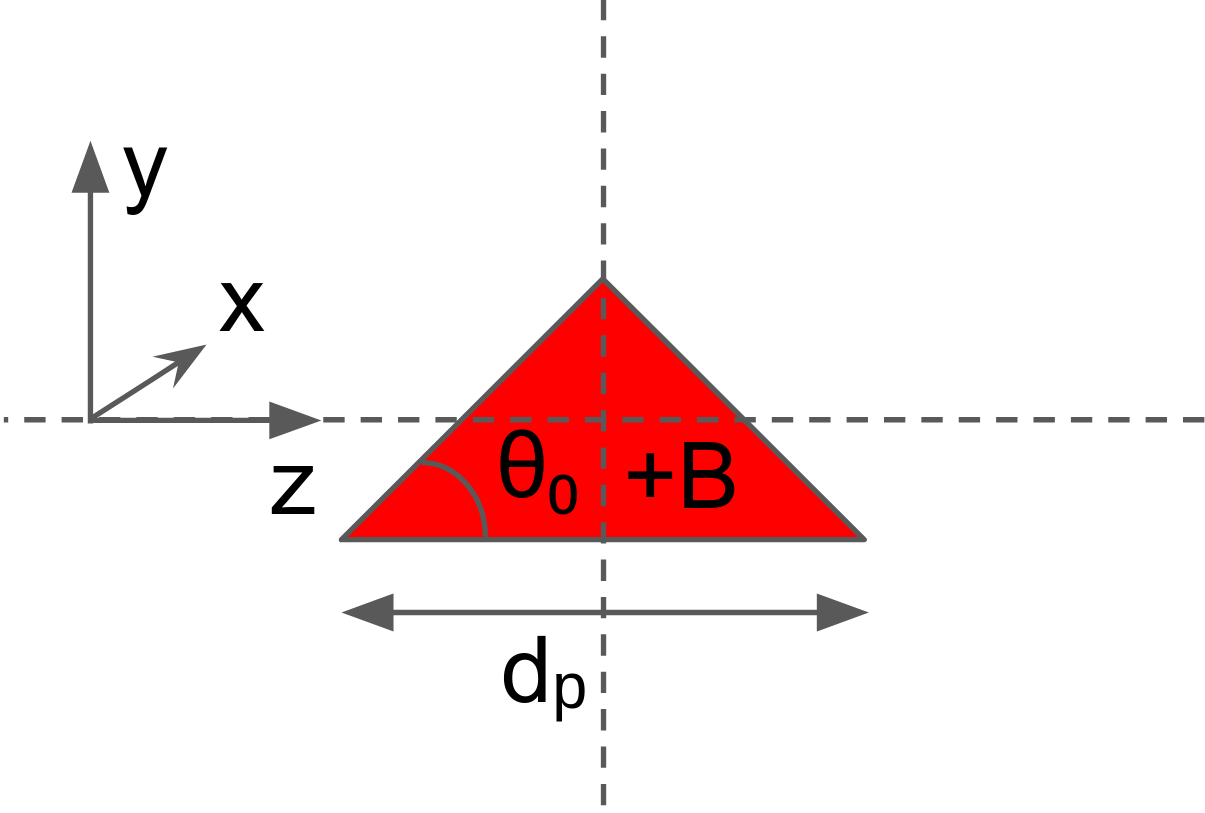
\includegraphics[width=\textwidth]{iso-schematic}
		\caption{Isosceles triangle.}
		\label{fig:precession-devices:iso}
	\end{subfigure}
	\hfill
	\begin{subfigure}[b]{0.3\textwidth}
		\centering
		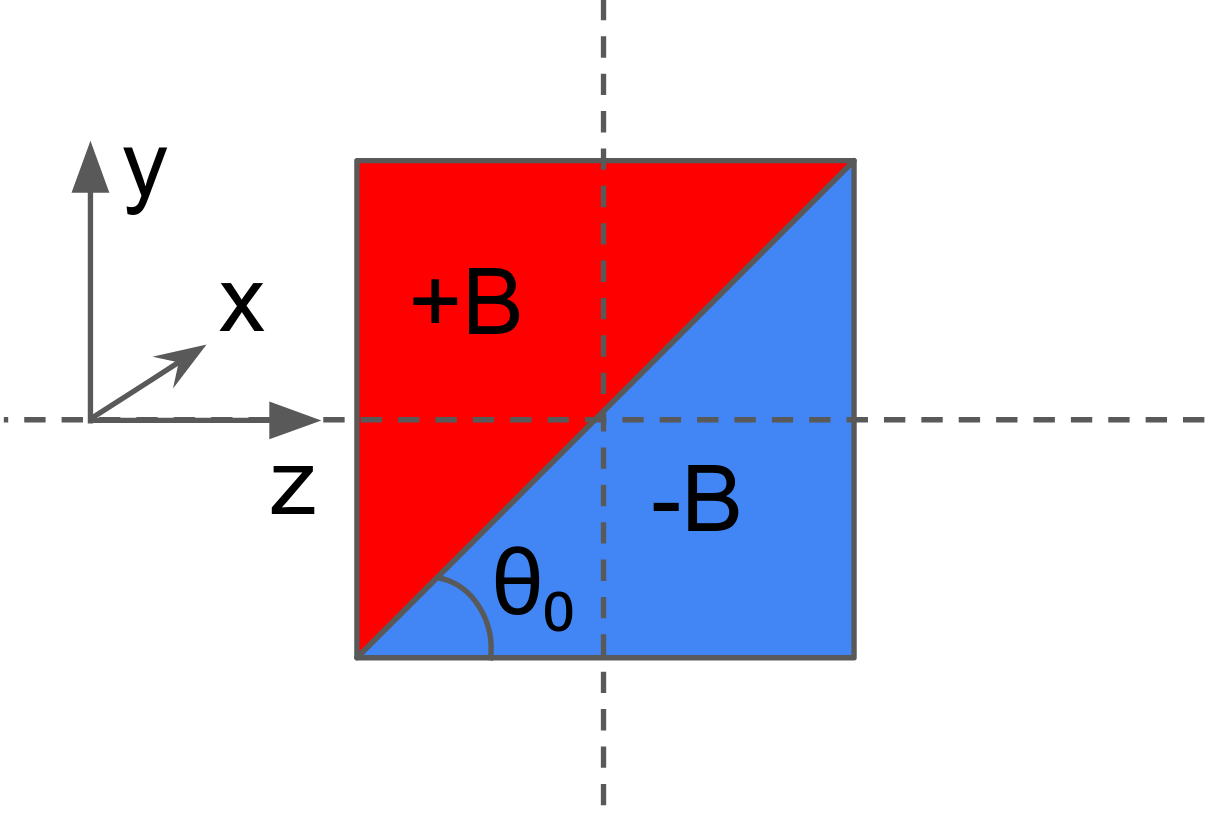
\includegraphics[width=\textwidth]{wp-schematic}
		\caption{Magnetic Wollaston prism.}
		\label{fig:precession-devices:wsp}
	\end{subfigure}
	\hfill
	\begin{subfigure}[b]{0.3\textwidth}
		\centering
		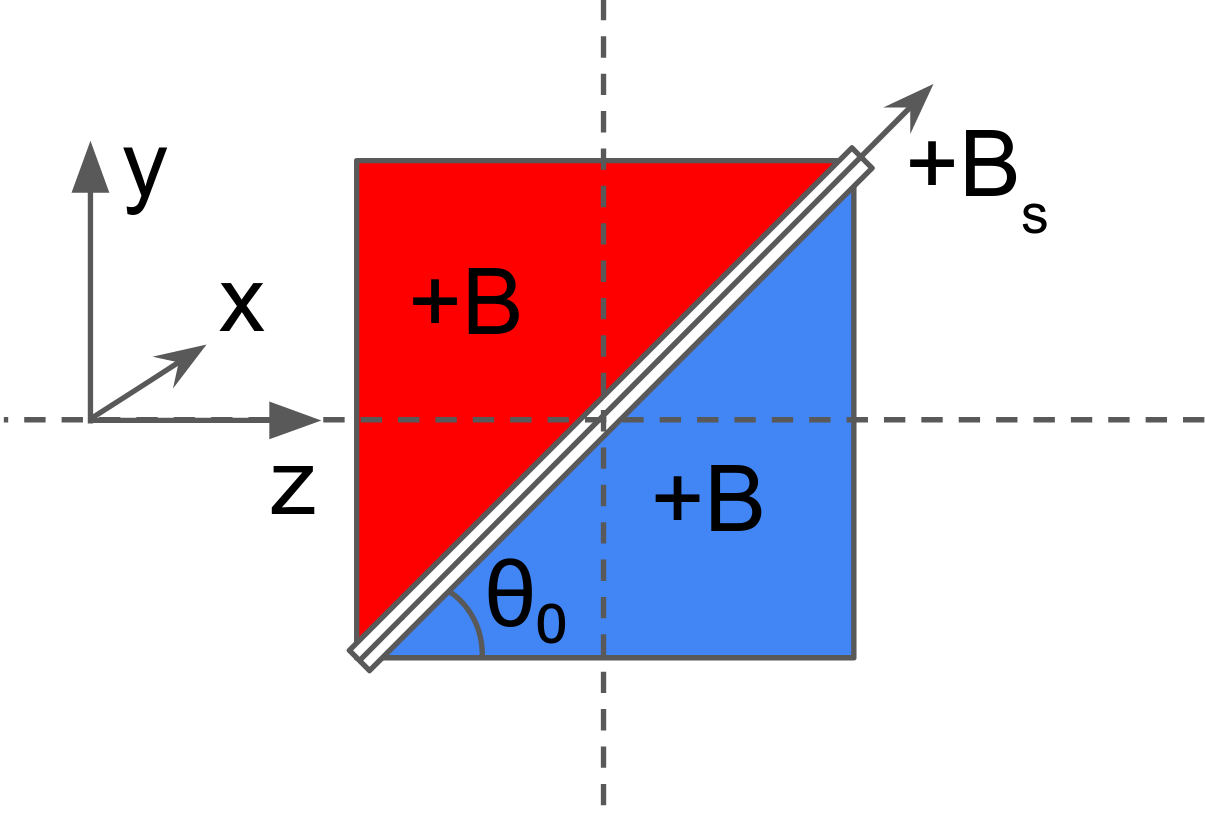
\includegraphics[width=\textwidth]{foil-schematic}
		\caption{Ferromagnetic foil flipper.}
		\label{fig:precession-devices:foil}
	\end{subfigure}
	\caption{Schematics for the three different types of precession devices. Assuming positive $B$, the red areas represent magnetic fields in the $+y$ direction, and the blue areas represent fields in the $-y$ direction, except in Figure \ref{fig:precession-devices:foil}. The reason for this is that the strong $B_s$ field inside the ferromagnetic foil effectively flips the precession of neutrons of the right $\lambda_0$, causing the positive field after the foil to have the effect of a negative field. This simulates the fields seen in a Wollaston prism as shown in Figure \ref{fig:precession-devices:wsp}. For all precession devices, the field interfaces are canted by $\theta_0$ in the $yz$-plane and all have depth $d_p = \SI{0.3}{\meter}$ as indicated in Subsection \ref{c3.3.4}. Only for Wollaston prisms $\theta_0 = \SI{45}{\deg}$ matching the angle shown in Figure \ref{fig:precession-devices:wsp}, with isosceles triangles in practice having $\theta_0 = \SI{20}{\deg}$ and $\theta_0$ being a function of $\lambda_0$ in the case of foil flippers.}
	\label{fig:precession-devices}
\end{figure}

\subsection{Device $\alpha$ and characteristics}
\label{c3.3.4}
To summarize the above discussion of the three available devices, once device-specific conditions are met a pair of any of them have in absolute terms the same precession-angle profile given by Equation \eqref{eq:precession-freq} with $\alpha = \frac{c(B_1 + B_2)}{\pi\tan\theta_0}$
\begin{equation}
	\phi = 2\pi\alpha\lambda y = \frac{2c\lambda (B_1 + B_2)y}{\tan\theta_0} \label{eq:device-prec}
\end{equation}
the contribution of each separate device being $\phi_i = \frac{2c\lambda B_i y}{\tan\theta_0}$. $\theta_0$ is a function of $\lambda_0$ for foil flippers and is fixed for Wollaston prisms and isosceles triangles, meaning that $B_1, B_2$ will in practice be set to vary $\alpha$. Table \ref{tab:device-properties} summarizes device characteristics as they appear in the literature that will be used in this research. All devices are assumed to have depth $d_p = \SI{0.3}{\meter}$, limiting possible values of $L_1, L_2$ and $L_s$. 
\begin{table}[h!]
	\centering
	\begin{tabular}{c|c c c c c}
		\toprule
		Name & Label & $\theta_0~[\unit{\degree}]$ & $B_{\text{min}}~[\unit{\milli\tesla}]$ & $B_{\text{max}} ~[\unit{\milli\tesla}]$ & Source \\
		\midrule
		Isosceles triangle & ISO & \num{20} & \num{0.1} & \num{15} & \cite{kusmin2017} \\
		Wollaston prism & WP & \num{45} & \num{0.1} & \num{63} & \cite{li2021} \\
		Foil flipper & FOIL & - & \num{0.3} & \num{30} & \cite{bouwman2011} \\
		\bottomrule
	\end{tabular}
	\caption{Precession device characteristics including the source of the values used. For a foil flipper, $\theta_0$ needs to be set to match $\lambda_0$ and is omitted. Its range is sufficient for all values of $\lambda_0$ considered in this research.}
	\label{tab:device-properties}
\end{table}
\subsection{Focussing condition}
In practice, neutrons will not travel parallel to the $z$-axis but move at a slight angle to this depending on beam divergence and other parameters. Letting $\psi$ be the angle their trajectory makes with the $z$-axis in the $yz$ plane, it can be seen that a neutron arriving at height $y$ on the detector will pass through the $i$'th precession device at average height $y_i = y + L_i\tan\psi \approx y + L_i\psi$, with $L_i$ being the distance from the detector of the device. This means that the total precession angle will be
$$\phi = 2c\lambda B_1\frac{y + L_1\psi}{\tan\theta_0} + 2c\lambda B_2\frac{y + L_2\psi}{\tan\theta_0}$$
This $\psi$-dependence is a problem as it will cause a loss of modulation depending on how large the variation in $\psi$ is. In first-order approximation, this effect can be removed by setting the positions $L_i$ and field strengths $B_i$ to meet the focussing condition
$$B_1L_1 = -B_2L_2$$
Substituting this retrieves Equation \eqref{eq:device-prec}. This gives also the motivation for using two devices: at least two are required to remove this $\psi$-dependency and achieve optimal modulation using a realistic, slightly divergent beam such as the one described above with $\psi_0 = \SI{2}{\milli\radian}$.
\section{Detector characteristics and $Q$-range}
\label{c3.4}
The position sensitive detector considered is $11\times11~\unit{\milli\meter}$ with a resolution of $1\times 1001$, so it has $1001$ pixels along the $y$-axis that integrate over the width of the detector. This corresponds to a pixel height of approximately $p = \SI{10.98}{\micro\meter}$ and a detector height $h_d = \SI{11}{\milli\meter}$. As the beam is focussed on the middle $10\times10~\unit{\milli\meter}$, this gives an effective detector height of $h_e = \SI{10}{\milli\meter}$. The modulation visibility with and without sample can be compared over this effective height $h_e$. As will be discussed in Chapter \ref{c4:constraints}, $h_e$ and $p$ limit the modulation frequencies $f = \alpha\lambda$ that can be sampled. 

The detector is placed at distance $L_s$ from the sample, meaning that ignoring divergence and assuming a straight beam, scattering from point $s_y = 0$ on the sample will be limited to angle $\theta_a = h_e/(2L_s)$ in small-angle approximation, resulting in a maximum wave-vector transfer of $Q_\text{max} \approx \frac{2\pi}{\lambda_0}\theta_a$. A fuller discussion of which angles are accepted by each point $y$ on the detector depending on beam collimation, sample size, and detector characteristics is given in \cite{kusmin2017}. Generally speaking, it can be seen that a detector can be used to integrate an experimental estimate $G_\text{exp}(\delta)$ of $G(\delta)$ as given in Equation \eqref{eq:G-analytical} limited by such a $Q_\text{max}$, given by 
\begin{equation}
	G_\text{exp}(\delta) = \frac{t}{k_0^2}\int_{-Q_\text{max}}^{Q_\text{max}}\int_{-Q_\text{max}}^{Q_\text{max}}\dfrac{d\sigma(\vec{Q})}{d\Omega}\cos(Q_y \delta)dQ_xdQ_y  \label{eq:G-experimental}
\end{equation}
assuming a symmetric detector with an equal $Q$-range for $x,y$. For samples with significant scattering with $Q > Q_{max}$, the error of $G_\text{exp}(\delta)$ as estimator of $G(\delta)$ can be expected to be significant whereas for samples with larger characteristic lengths and scattering over lower $Q$-ranges, the error will be negligible with most scattered neutrons being picked up by the detector \cite{rekveldt1996} so that $G_\text{exp}(\delta)$ approximates $G(\delta)$ well. 

\section{The sample and its position $L_s$}
\label{c3.5}
The model sample that is considered in this work is a dilute mono-disperse solution of solid spheres as described in Section \ref{c2.4} with radii varying from $R = \SI{50}{\nano\meter}$ to $R = \SI{2000}{\nano\meter}$. It is modeled as a $20\times20~\unit{\milli\meter}$ square with thickness $t$ along the $z$-axis, meaning that it is significantly wider than the beam as described above. 

In general, the distance from the sample to the detector $L_s$ can be varied in a given instrument to measure different samples and this is done in practical SEMSANS instrument designs \cite{kusmin2017}. However, as mentioned in Section \ref{c1.3}, one of the target applications of the instrument is to study processes in colloids like milk turning into yogurt which encompass the full target range of $\SI{10}{\nano\meter}$ to $\SI{5}{\micro\meter}$. This means that it is not practical to adjust $L_s$ in the middle of measurements as it would require precise remote control of the sample holder. It is assumed that such control is not available in this model and that for a given sample measurement $L_s$ is fixed, although measurements can be performed at different $L_s$.  

\subsection{Permissible sample positions $L_s$}
When positioning a sample in an instrument, an important criterion is that $h_e/L_s$ needs to be small enough so that the small-angle approximation $Q_{max} \approx \frac{2\pi}{\lambda_0}\frac{h_e}{2L_s}$ remains valid. Assuming elastic scattering, the third-order approximation of $Q_{max}$ is given by
$$Q_{max} = \frac{4\pi}{\lambda_0}\sin(\frac{\arctan\frac{h_e}{2L_s}}{2}) \approx  \frac{2\pi}{\lambda_0}(\frac{h_e}{2L_s} - \frac{3h_e^3}{64L_s^3})$$
making the relative approximation error proportional to $\epsilon_\angle = \frac{3h_e^2}{32L_s^2}$. What values of $h_e/L_s$ and $\epsilon_\angle$ are permissible is unclear as no studies have been done investigating this specifically. Values like $\theta_a \approx \SI{30}{\milli\radian}$ are used in SESANS \cite{rekveldt1996}, but it is not obvious if this can be translated to a SEMSANS acceptance angle. To be on the safe side, $\theta_a = \arctan\left(h_e / (2L_s)\right) = \SI{15}{\milli\radian}$ will be used as an upper limit, translating to a lower limit of $L_{s,min} = \SI{0.333}{\meter}$ for $h_e = \SI{10}{\milli\meter}$ with $\epsilon_\angle = \num{8.4e-5}$. 
The upper limit of $L_s$ is determined by the depth of the second precession device $d_p$, its position $L_2$ and sample thickness $t$, giving $L_{s,max} = L_2 - d_p / 2 - t/2$. Assuming a maximal sample depth of $t=\SI{0.01}{\meter}$, this evaluates to $L_{s,max} = 1.845 \approx \SI{1.8}{\meter}$. Factors like analyzer and sample holder dimensions will in practice further limit $L_s$ but this is ignored in this simple model.
\section{Polychromatic SEMSANS}
\label{c3.6}
The usual description of SEMSANS modulation patterns as given in \eqref{eq:mono-modulation} and their relation to a spin-echo length \eqref{eq:delta} typically assumes a monochromatic source or a source that closely approximates it, for instance by using a PG monochromator with $\Delta\lambda/\lambda_0 = 0.01$ with thermal neutrons. However, even then a modulation envelope can be seen to appear \cite{bouwman2021} due to this wavelength spread. This effect becomes far more important when using a velocity selector with $\Delta\lambda/\lambda_0 = 0.1$ to select a higher wavelength such as $\lambda_0 = \SI{8}{\angstrom}$ and is here discussed in detail.
\subsection{Modulation envelope for Gaussian $\lambda$ spectrum}
Assuming a Gaussian wavelength distribution as given by Equation \eqref{eq:gauss-spectrum} and neglecting wavelength-specific effects like foil flipper polarization loss, it can be shown using Fourier analysis that the base intensity modulation becomes
\begin{equation}
	I_b(y) = I_{0,b} \pm A_bE(y)\cos(2\pi\alpha\lambda_0y) \label{eq:poly-base-modulation}
\end{equation}
The envelope $E(y)$ is a Gaussian and given by
\begin{equation}
	E(y) = e^{-\frac{1}{2}\left(2\pi\alpha\sigma y\right)^2} \label{eq:poly-base-modulation-env}
\end{equation}
Substituting $\sigma=0$ for a monochromatic limit gives back Equation \eqref{eq:mono-modulation}. This modulation envelope $E(y)$ can be shown to have a FWHM of
\begin{equation}
	FWHM_E = \frac{\sqrt{2\ln 2}}{\pi\alpha\sigma} \label{eq:poly-base-modulation-fwhm}
\end{equation}
It follows that increasing wavelength spread $\sigma$ results in a narrower modulation envelope width. It also confirms the envelope narrowing observed when increasing $B$-field strengths \cite{bouwman2021} as it is a function of $\alpha$. 
\subsection{Effect on interaction with sample and $\delta$-resolution}
At first glance, it is clear that the effect of a sample on the modulation will be more complicated than a simple reduction of the amplitude of the modulation envelope. The modulation now consists of a range of wavelengths $\lambda$, each related to a spin-echo length $\delta = \lambda^2 L_s\alpha$ and each with a scattering power $\tau \propto\lambda^2$ such as Equation \eqref{eq:sample-tau}. Although Equations \eqref{eq:mono-modulation} and \eqref{eq:sample-pol-reduction} by itself do not describe the corresponding modulation pattern, they do describe what happens to a single frequency so that
\begin{equation}
	I_s(y) = I_{0,s} + \int_{-\infty}^\infty f_{\text{gauss}}(\lambda)e^{G(\lambda^2 L_s\alpha) - \tau(\lambda)}A_b\cos(2\pi\alpha\lambda y)d\lambda \label{eq:poly-sample-modulation}
\end{equation}
per linearity describes the modulation pattern. Qualitatively it can be seen that for greater $\sigma$, a greater $\delta$-range is accessed around a central value $\delta_0 = \lambda_0^2L_s\alpha$ and this is reflected in the Fourier spectrum of $I_s(y)$. The width of this $\delta$-range is proportional to $\delta_0$, meaning that the potential effect it has on resolution is relative rather than absolute. This means that estimating $G(\delta_0)$ from the visibility of the intensity modulation described by Equation \ref{eq:poly-sample-modulation} will introduce error depending on the specific sample. One way to avoid this problem is to consider the effect of the sample in the frequency domain using Fourier analysis. This does bring with it new problems such as frequency resolution limitations when estimating the spectrum.


\section{Instrument design variants}
\label{c3.7}
Using the basic instrument model described and analyzed in this chapter, with the various options in terms of monochromators and precession devices, a few design variants can be formulated combining the different options for these component types. Firstly, there is the choice of $\lambda_0$ and the corresponding monochromator. Two considered values are $\lambda_0 = \SI{4.321}{\angstrom}$ with a PG monochromator giving $\Delta\lambda = \SI{0.04321}{\angstrom}$ and $\lambda_0 = \SI{8}{\angstrom}$ with a velocity selector giving $\Delta\lambda = \SI{0.8}{\angstrom}$. These two sources are combined with each of the three precession devices as characterized in Table \ref{tab:device-properties}, giving Table \ref{tab:design-variants} which includes the appropriate $\theta_0$ needed to achieve $\phi_{foil} = \pi$ in the case of foil flippers. These instruments will first be analyzed in the next chapter to estimate their $\delta$-range by using constraints as well as their estimated intensity. In Chapter \ref{c6:monte-carlo}, Monte Carlo simulations of measurements using these instruments are discussed.

What the designs have in common are the precession device positions $L_1 = \SI{4.0}{\meter}, L_2 = \SI{2.0}{\meter}$. Additionally, the detector dimensions are $11\times 11~\unit{\milli\meter}$ with pixel size $p = \SI{10.98}{\micro\meter}$ and the distance from source to detector is $d = \SI{5}{\meter}$, summarizing from what is given above. The beam dimensions at the detector are $10\times 10~\unit{\milli\meter}$, giving an effective detector height of $h_e =\SI{10}{\milli\meter}$. For simplicity and to facilitate comparison, the approximate maximum value of $L_s = \SI{1.8}{\meter}$ will be used in all calculations for the designs, including the computed constraints in Chapter \ref{c4:constraints} and the Monte Carlo simulations presented in Chapter \ref{c6:monte-carlo}. The possibility of optimizing distances $L_1, L_2, L_s$ together with $\lambda_0$ for a given choice of monochromator and precession device is discussed in Chapter \ref{c5:optimization}.  

\begin{table}[h!]
	\centering
	\begin{tabular}{ c|c c c | c c c c }
		\toprule
		Label & $\lambda_0~[\unit{\angstrom}]$ & $\Delta\lambda~[\unit{\angstrom}]$ & Monochromator & Device & $\theta_0~[\unit{\degree}]$ & $B_{\text{min}}~[\unit{\milli\tesla}]$ & $B_{\text{max}} ~[\unit{\milli\tesla}]$ \\
		\midrule
		ISO 4.321 & \num{4.321} & \num{0.04321} & PG & ISO & \num{20} & \num{0.1} & \num{15} \\
		WP 4.321 & \num{4.321} & \num{0.04321} & PG & WP & \num{45} & \num{0.1} & \num{63} \\
		FOIL 4.321 & \num{4.321} & \num{0.04321} & PG & FOIL & \num{11.013} & \num{0.3} & \num{30} \\
		ISO 8 & \num{8} & \num{0.8} & VS & ISO & \num{20} & \num{0.1} & \num{15} \\
		WP 8 & \num{8} & \num{0.8} & VS & WP & \num{45} & \num{0.1} & \num{63} \\
		FOIL 8 & \num{8} & \num{0.8} & VS & FOIL & \num{20.714} & \num{0.3} & \num{30} \\
		
		\bottomrule
	\end{tabular}
	\caption{Six SEMSANS instrument design variants combining two $\lambda_0$ and monochromator pairings with three precession device types. Designs are labeled by combining their device type and the value of $\lambda_0$ in Å.}
	\label{tab:design-variants}
\end{table}

\chapter{$\delta$-constraints and intensity in instrument design}
\label{chapter:constraints}
\label{c4:constraints}
Two key parameters in SEMSANS instrument design are the accessible $\delta$-range and the intensity at the detector. The first determines the range of samples that can be measured and the second the amount of signal per unit time, which determines how well you can measure in given time or similarly the measurement time needed for a required measurement quality. In this chapter, building on the analysis presented in Chapter \ref{c3}, a system of constraints will be presented that together limit the accessible $\delta$ range for each of the designs listed in Table \ref{tab:design-variants}. After discussing the $\delta$-ranges, a coarse estimate for the intensity at the detector for the two source options will be presented. Lastly, the effect of intensity loss due to SANS scattering is discussed by using a very primitive model for scattering based on the sample form factor $P(Q)$, the goal being to understand the lower $\delta$-limit of the presented instruments better.
\section{Constraints}
\label{c4.1}
Three main sources of limitations can be recognized. Firstly, the effective detector height $h_e$ and pixel size $p$ as well as the distance from detector to sample $L_s$ will limit which modulation frequencies can be sampled as well as the accessible $Q$-range, limiting $\delta$ in various ways.
Secondly, the mean wavelength $\lambda_0$ as well as the monochromator quality $\frac{d\lambda}{\lambda_0}$ (and corresponding wavelength $\sigma$) shape the modulation envelope and determine how quickly it will become too narrow as $\alpha$ increases due to increasing field strengths, with $\lambda_0$ also playing a role in all other bounds. Lastly, the basic characteristics of precession devices as well as their positions relative to the detector limit the range of $\alpha$ and how strong the precession gradient is along the $y$-axis. 

% Discuss sources of constraints, linking them to the theory in previous chapters. Ideally refer to equation numbers to avoid repetition and make it sound really solid. 
% Emphasize that these constraints serve as a starting point for estimating limitations for given instruments
\subsection{Detector sampling limitations}
Using detector sampling frequency $f_s = \frac{1}{p}$, the Nyquist frequency is $f_n = f_s/2$ and this an exclusive upper-limit at two samples per modulation period, corresponding to 
$$\delta_{max,n} = \frac{\lambda_0L_s}{2p}$$
This can be derived from the form of $\delta$ that is independent of $\alpha$, $\delta = \lambda_0 fL_s$. In practice, modulation visibility is reduced when approaching this frequency. One way to reduce this is to set a bound for this effect and solve it numerically as done in \cite{kusmin2017}. A simple alternative to this is to require more samples per period, for instance $5$ instead of $2$ giving
$$\delta_{max,s} = \frac{\lambda_0L_s}{5p}$$
Similarly, the requirement that at least 1 modulation period is visible on the detector restricts the frequency to a minimum of $f_{min} = \frac{1}{h_e}$, corresponding to 
$$\delta_{min,s} = \frac{\lambda_0L_s}{h_e}$$
An alternative and equivalent way of deriving this is through considering the detected $Q$-range, using $Q_{max}$ and $\theta_a$ as described in Section \ref{c3.4}. This gives 
$$Q_{max} = \frac{\pi h_s}{\lambda_0 L_s}$$
This is equivalent to $\delta_{min,s}$ as it satisfies $\delta_{min,s} Q_{max} = \pi$. It also provides an idea of the $Q$-range that reaches the detector, providing a coarse upper limit for $Q$ and accessible characteristic sample lengths. 

\subsection{Modulation envelope width}
As discussed before, the modulation can be described by a Gaussian envelope with a FWHM as given by Equation \eqref{eq:poly-base-modulation-fwhm}. Using $\delta = \lambda_0^2L_s\alpha$ and given a $FWHM_{e,min}$, this can be rewritten to a maximum $\delta$ value
$$\delta_{max,e} = \frac{\sqrt{2\ln 2}\lambda_0^2 L_s}{\pi\sigma FWHM_{e,min}}$$
In this way, the intuitive notion that the envelope should not become too narrow to measure enough signal can be translated to a concrete limit by choosing $FWHM_{e,min}$. For monochromators with a low $\Delta\lambda$ and a corresponding low $\sigma$ such as PG monochromators, this will in practice not normally be a limit but it can be when using velocity selectors. The chosen value in this work for $FWHM_{e,min}$ is $\SI{2}{\milli\meter}$, so $20$\% of the effective detector height $h_e$ and it is somewhat permissive.  

\subsection{Precession device limitations}
In terms of instrument design, the engineering of precession devices with a high $\alpha$ and optimizing their positions from the detector $L_1, L_2$ perhaps has the greatest impact on $\delta$-range. The importance of $L_1, L_2$ comes from the focussing condition, which is $B_1L_1 = -B_2L_2$ for two devices. As $\alpha\propto B_1 + B_2$ and $B_1, B_2$ are each limited by device-specific $B_{min}, B_{max}$ as given by Table \ref{tab:device-properties}, $B_1 + B_2$ is bounded by
$$(B_1 + B_2)_{min} = (\frac{L_1}{L_2} - 1)B_{min}$$
$$(B_1 + B_2)_{max} = (1 - \frac{L_2}{L_1})B_{max}$$
For the minimum value, $B_1 = B_{min}$ and for the maximum value, $B_2 = B_{max}$ with the other set accordingly. Using $\alpha = \frac{c(B_1+B_2)}{\pi\tan\theta_0}$, the following $\delta$ constraints can be derived
$$\delta_{min, f} = \lambda_0^2 L_s \frac{c(\frac{L_1}{L_2} - 1)B_{min}}{\pi\tan\theta_0}$$
$$\delta_{max, f} = \lambda_0^2 L_s \frac{c(1 - \frac{L_2}{L_1})B_{max}}{\pi\tan\theta_0}$$

\begin{table}[h!]
	\centering
	\begin{tabular}{c | c c | c c c}
		\toprule
		Label & $\delta_{\text{min,s}}$ (nm) & $\delta_{\text{min,d}}$ (nm) & $\delta_{\text{max,s}}$ (nm) & $\delta_{\text{max,e}}$ (nm) & $\delta_{\text{max,d}}$ (nm) \\
		\midrule
		FOIL 4.321 & \textbf{77.8} & \num{76.3} & \num{14.2} & \num{34.3} & \textbf{3.82} \\
		WSP 4.321 & \textbf{77.8} & \num{5.00} & \num{14.2} & \num{34.3} & \textbf{1.56} \\
		ISO 4.321 & \textbf{77.8} & \num{13.6} & \num{14.2} & \num{34.3} & \textbf{1.02} \\
		FOIL 8 & \textbf{144} & \num{135} & \num{26.2} & \textbf{6.35} & \num{6.73} \\
		WSP 8 & \textbf{144} & \num{17.0} & \num{26.2} & \num{6.35} & \textbf{5.35} \\
		ISO 8 & \textbf{144} & \num{46.6} & \num{26.2} & \num{6.35} & \textbf{3.50} \\
		\bottomrule
	\end{tabular}
	\caption{Calculated $\delta$ constraints for the designs with the constraints limiting the final $\delta$-range listed in Table \ref{tab:designs-final-ranges} marked in bold for each design.}
	\label{tab:designs-delta-constraints}
\end{table}
\section{Computed $\delta$ constraints and design $\delta$ ranges}
\label{c4.2}
The computed $\delta$-constraints for the designs are given in Table \ref{tab:designs-delta-constraints}. From these together, $\delta$-ranges can be calculated for each design as given in Table \ref{tab:designs-final-ranges} together with their $Q_{max}$. %These values were computed using $L_s = 1.8\unit\meter$, which is approximately the maximal $L_s$ setting available. This means that shorter $\delta_{min}$ is accessible by reducing $L_s$ but $\delta_{max}$ is the maximal spin-echo length that can be measured.
\begin{table}[h!]
	\centering
	\begin{tabular}{c | c c c c | cc}
		\toprule
		Label & $Q_{\text{max}} ~[\unit{\angstrom^{-1}}]$ & $\theta_a~[\unit{\milli\radian}]$ & $\delta_{min}~[\unit{\nano\meter}]$ & $\delta_{max}~[\unit{\micro\meter}]$ & $\delta_{min,abs}~[\unit{\nano\meter}]$ & $\delta_{max,abs}~[\unit{\micro\meter}]$ \\
		\midrule
FOIL 4.321 & \num{0.00404} & \num{2.78} & \num{77.8} & \num{3.82} & \num{14.4} & \num{3.91} \\
WSP 4.321 & \num{0.00404} & \num{2.78} & \num{77.8} & \num{1.56} & \num{14.4} & \num{1.60} \\
ISO 4.321 & \num{0.00404} & \num{2.78} & \num{77.8} & \num{1.02} & \num{14.4} & \num{1.05} \\
FOIL 8 & \num{0.00218} & \num{2.78} & \num{144.} & \num{6.35} & \num{26.7} & \num{6.51} \\
WSP 8 & \num{0.00218} & \num{2.78} & \num{144.} & \num{5.35} & \num{26.7} & \num{5.48} \\
ISO 8 & \num{0.00218} & \num{2.78} & \num{144.} & \num{3.50} & \num{26.7} & \num{3.59} \\
		\bottomrule
	\end{tabular}
	\caption{Key characteristics for the various designs, with $\delta_{min}, \delta_{max}$ being computed using the constraints listed in Table \ref{tab:designs-delta-constraints}. Also included are $\delta_{min,abs}, \delta_{max,abs}$ which indicate the absolute limits that can be measured using $L_s = L_{s,min} = \SI{0.333}{\meter}$ and $L_s = L_{s,max} = \SI{1.84}{\meter}$ respectively}
	\label{tab:designs-final-ranges}
\end{table}
\subsection{Discussion of design constraints}
The computed $\delta$-ranges and $Q_{max}$ give a first understanding of for what samples the designs can be used to estimate $G(\delta)$ through $G_{\text{exp}}(\delta)$. $\delta$ limits the range of $G(\delta)$'s that can be estimated and $Q_{max}$ gives an indication of how well the bounded integral will approximate the true value. It can be seen that instruments at $\lambda_0 = \SI{4.321}{\angstrom}$ have a wider $Q$-range given the same $L_s, h_e$ as was to be expected from $Q_{max} \propto 1/\lambda_0$ and correspondingly a lower $\delta_{min}$, making them better able to characterize samples of $\delta \approx \SI{100}{\nano\meter}$. For instruments with triangles and prisms, the condition that at least one modulation period must fit on the detector with effective height $h_e$ is a limiting factor, whereas for foils the devices and their positions $L_1, L_2$ limit $\delta$. Another observation that can be made is that instruments at $\lambda_0 = \SI{4.321}{\angstrom}$ with a narrower $\lambda$ spectrum are limited more strongly by the upper sampling limit due to detector pixel size $p$ whereas with a wider spectrum at $\lambda_0 = \SI{8}{\angstrom}$ the narrowing of the modulation envelope becomes a limiting factor. With exception of FOIL 8, the upper $\delta$ limit is in these instruments determined by device characteristics together with $L_1, L_2, L_s$ as well as the specific $\lambda_0$ operating point. 


\subsection{Limitations of constraint scheme}
Together, the constraints above give an impression of various factors limiting the achievable $\delta$-range for SEMSANS instruments with $2$ precession devices. It makes it possible to quickly evaluate designs such as those given and identify possibilities to improve them by making the necessary changes. There are some key limitations however, in particular related to the beam and the detector $Q$-range. As mentioned in Section \ref{c3.4} it is assumed that the beam covers an effective detector height of $h_e$ which translates to requirements for the beam width and/or divergence. The intensity across the beam is assumed to be uniform, which means that the used Gaussian modulation pattern might be too simple of a model for the modulation envelope. As for the $Q$-range, the lower limit imposed by sampling and the precession devices might be too permissive as in practice at the smallest $\delta$, $Q_{max}$ can be too low and $G_\text{exp}(\delta)$ can significantly deviate from $G(\delta)$, this will be discussed in Section \ref{c4.4}. $B$-resolution limitations and how these could influence the $\delta$-resolution were also not considered. Lastly, all computed constraints are derived from values as listed in Table \ref{tab:device-properties} and elsewhere meaning that if say improved precession devices are available with greater $B_{max}$ or different $\theta_0$, the constraints need to be reevaluated.  
%Some factors that were not taken into account are errors in $G_\text{exp}$ for the lowest $\delta$ values where the $Q$-range might be insufficient as well as more acc


% Discuss things that are missing
%Also very important: discuss the softer constraints: why should the envelope FWHM be 3mm and not 2mm or 4mm? What determines this other than vibes. Indicate how they could be made more/less flexible		




\section{Intensity estimate}
\label{c4.3}
In this section, a coarse estimate of intensities as they can be expected using the described designs is derived. Although accurate intensity estimates are beyond the scope of this research, requiring detailed characterizations of losses in all components as well detailed information about the newly installed cold source, a highly simplified estimate assuming ideal components can be derived as follows.

The original targetted value for the full-spectrum flux at the new cold source beamline corresponding to a reactor power of $\SI{3}{\mega\watt}$ of $\SI{1e9}{\centi\meter^{-2}\sec^{-1}}$ \cite{OYSTER2008} is taken as a starting point. It is assumed that the intensity of the source has about half the original targetted intensity, so $\Phi_0 = \SI{5e8}{\centi\meter^{-2}\sec^{-1}}$. Given an operating point $\lambda_0$ with a matching $\sigma$ from the monochromator type, the intensity can be estimated by numerical evaluation of the integral
$$\Phi_{mc} \propto \int_0^\infty f_\lambda(\lambda)e^{-\frac{1}{2}\left(\frac{\lambda - \lambda_0}{\sigma}\right)^2}d\lambda \Phi_0= C_{mc}\Phi_0$$
The transfer of the monochromator is assumed to be a lossless Gaussian, and losses from beam divergence from beamline to monochromator are neglected.  It can easily be seen from Figure \ref{fig:source-spectrum} that the choice of $\lambda_0$ matters here, as well as the value of $\sigma$. For the used monochromators at $\lambda_0 = \SI{4.321}{\angstrom}$ and $\lambda_0 = \SI{8}{\angstrom}$ with $\Delta\lambda = \SI{0.4321}{\angstrom}$ and $\Delta\lambda = \SI{0.8}{\angstrom}$ the integral on the left evaluates to $C_{mc} = 0.00631826$ and $C_{mc} = 0.07346646$. Assuming an ideal polariser and an ideal analyser, the average loss of intensity for $\pm x$ analyser settings due to these corresponds to a factor $1/4$. To account for losses due to beam divergence, consider the beam divergence to be a small angle $\psi_0$. 
For a uniform beam of radius $R_0$ coming out of the beamline with such a divergence $\phi_0$, it will have expanded to radius $R = R_0 + \psi_0 d$ in small-angle approximation. Simplifying the distribution of neutrons to be uniform over this radius after expansion, the flux at distance $d$ behind the analyser can be seen to be proportional to
$$\Phi(d) \propto \frac{\Phi_{mc}}{4}\frac{R_0^2}{(R_0 + \psi_0 d)^2} = \frac{\Phi_0}{4}C_{mc}C_{div}$$
Consider $R = \SI{0.1}{\meter}$ to be the radius of the beamline and let $\phi_0 = \SI{2}{\deg}$. Using $d = \SI{6}{\meter}$ as estimate for the distance of the sample to the beamline gives a divergence loss factor of about $C_{div} = 0.1044$.

Using this approach gives highly optimistic order of magnitude estimates of the flux at the sample for both $\lambda_0$ options: $100021 \approx \SI{1e5}{\centi\meter^{-2}\sec^{-1}}$ and $959064 \approx \SI{1e6}{\centi\meter^{-2}\sec^{-1}}$ for $\lambda_0 = \SI{4.321}{\angstrom}$ and $\lambda_0 = \SI{8}{\angstrom}$ respectively, the order of magnitude difference being due to the greater $\Delta\lambda/\lambda_0$ of the velocity selector compared to the PG crystal under the assumption of an optimal Gaussian transfer. As the detector has an area of approximately $\SI{1}{\centi\meter^2}$ and neglecting additional losses due to further divergence, this is also roughly the total intensity at the detector, at least in the absence of a sample or when using a sample that scatters only into a very small $Q$-range. Various losses due to non-ideal components etc. can be expected to reduce these estimates by perhaps another of magnitude and the relative efficiency of concrete PG and VS monochromators could cancel the estimated benefit of the VS.

\section{Sample scattering and intensity}
\label{c4.4}
Although so far the the accessible $\delta$-range and detector intensity have been discussed separately, the characteristic length of the sample measured will have a tangible effect on the measured intensity as well as the quality of $G_{exp}(\delta)$ as estimate of $G(\delta)$ limited to $Q_{max}$ for lower $\delta$ and higher $\lambda_0$. This effect was first discussed in the context of SESANS with an instrument for which $\lambda_0 =  \SI{2}{\angstrom}$ and $\theta_a \approx \SI{30}{\milli\radian}$ \cite{rekveldt1996}, where it was concluded that for characteristic lengths larger than $\SI{5}{\nano\meter}$ SESANS can be used to reliably estimate $G(\delta)$. Using $L_s = \SI{1.8}{\meter}$ for the instruments considered here, $\theta_a \approx h_e / (2L_s) = \SI{2.8}{\milli\radian}$. With $\lambda_0 = \SI{4.321}{\angstrom}$ and $\lambda_0 =  \SI{8}{\angstrom}$, this estimated limit translates to about $\SI{100}{\nano\meter}$ and $\SI{200}{\nano\meter}$ respectively. This indicates that the true $\delta$-range might be more limited using current $h_e,L_s$ and the colder wavelengths. This effect is here verified using a very primitive non-randomized computational approach from which deviation from the ideal regime in which almost all scattered neutrons reach the detector \cite{rekveldt1996} can be seen. 
\begin{figure}[htbp]
	\centering
	\begin{subfigure}[b]{0.49\textwidth}
		\centering
		\includegraphics[width=\textwidth]{simplified-I-scattering-3D-plot-point-4.321}
		\caption{Scattering from point $(s_x,s_y) = (0,0)$ projected onto the detector plane.}
		\label{fig:simplified-scattering-3D:a}
	\end{subfigure}
	\hfill
	\begin{subfigure}[b]{0.49\textwidth}
		\centering
		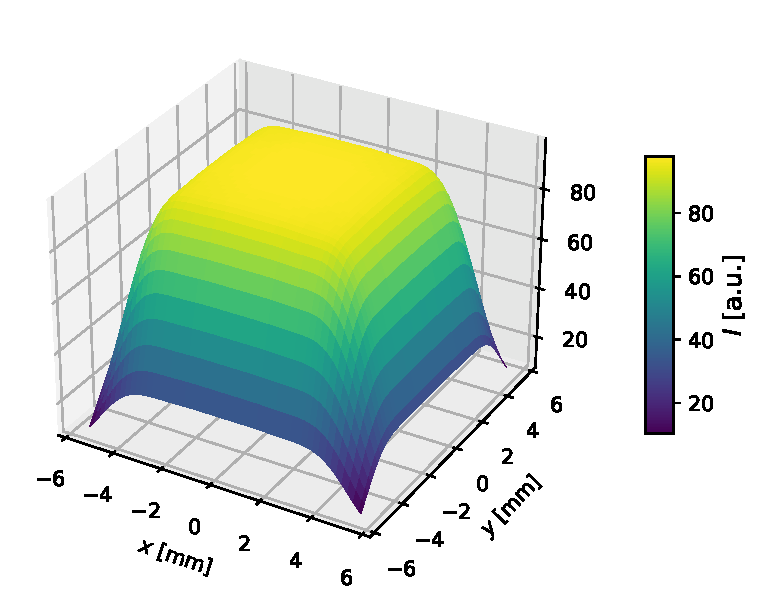
\includegraphics[width=\textwidth]{simplified-I-scattering-3D-plot-4.321}
		\caption{Scattering integrated over entire sample and normalized.}
		\label{fig:simplified-scattering-3D:b}
	\end{subfigure}
	\caption{An illustration of a simple scattering model assuming a very thin sample and single scattering of a square beam with $R= \SI{200}{\nano\meter}$, $\lambda_0 =  \SI{4.321}{\angstrom}$ and $L_s = \SI{1.8}{\meter}$. Beam divergence is neglected and a uniform profile is assumed. Figure \ref{fig:simplified-scattering-3D:a} shows the intensity contribution of a single point $(s_x,s_y) = (0,0)$ projected onto the detector. Figure \ref{fig:simplified-scattering-3D:b} shows the normalized result of integrating over the full $10\times10~\unit{\milli\meter}$ sample, giving an indication of how much of the scattered fraction of neutrons is detected and which part of the detector can be used to reliably compute $G_\text{exp}$ without resorting to Monte Carlo methods.}
	\label{fig:simplified-scattering-3D}
\end{figure}
\begin{figure}[htbp]
	\centering
	\begin{subfigure}[b]{0.49\textwidth}
		\centering
		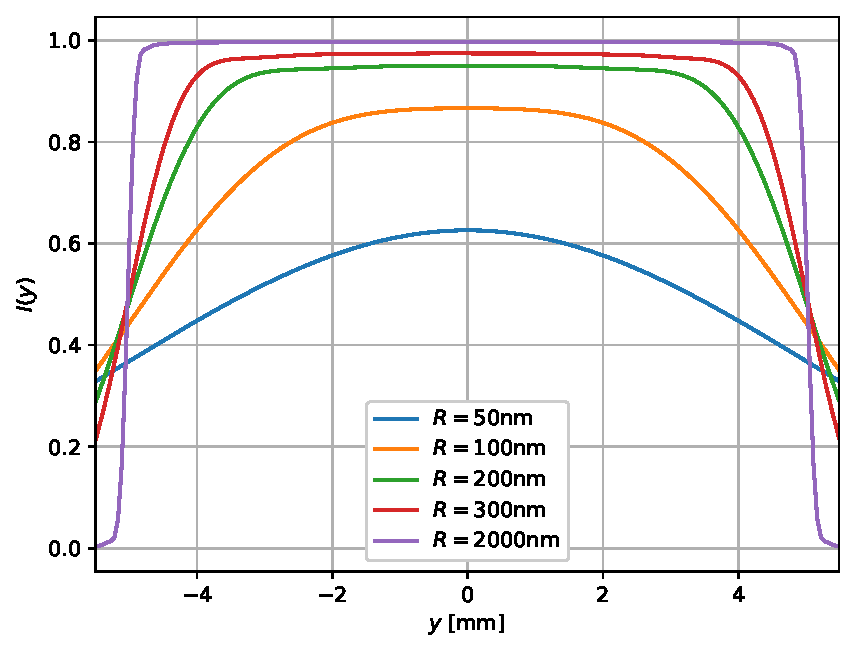
\includegraphics[width=\textwidth]{simplified-I-scattering-4.321}
		\caption{Estimated detected scattering fraction for $\lambda_0 = \SI{4.321}{\angstrom}$}
		\label{fig:simplified-scattering-4.321}
	\end{subfigure}
	\hfill
	\begin{subfigure}[b]{0.49\textwidth}
		\centering
		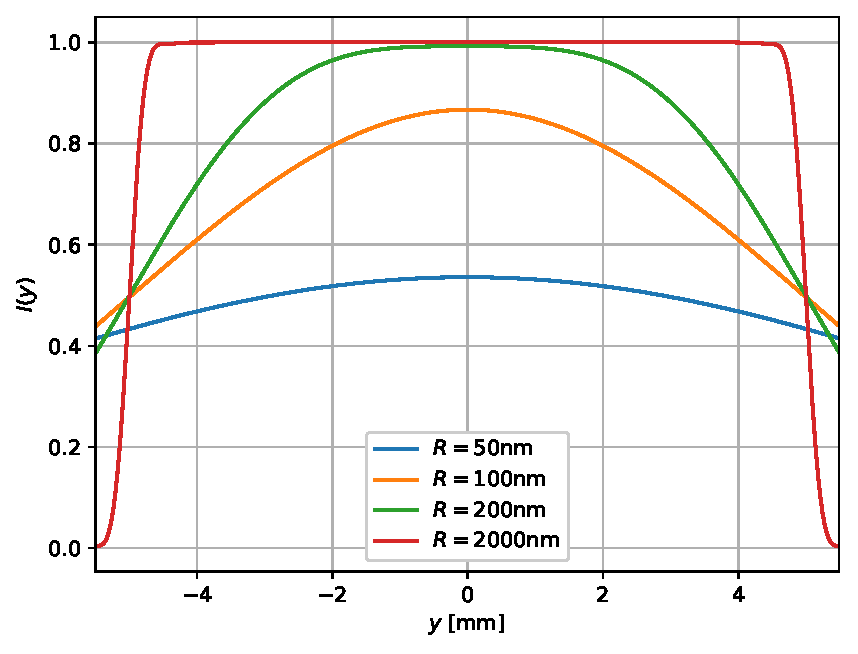
\includegraphics[width=\textwidth]{simplified-I-scattering-8.0}
		\caption{Estimated detected scattering fraction for $\lambda_0 = \SI{8}{\angstrom}$}
		\label{fig:simplified-scattering-8}
	\end{subfigure}
	\caption{A comparison of the estimated fraction of scattered neutrons that is detected at each point on the detector with $L_s = \SI{1.8}{\meter}$ for $\lambda_0 = \SI{4.321}{\angstrom}$ and $\lambda_0 = \SI{8}{\angstrom}$ and different radii $R$. Curves are calculated by first computing a 2D intensity pattern as illustrated in Figure \ref{fig:simplified-scattering-3D:b}, after which the pattern is integrated over $x$ and normalized.} 
	\label{fig:simplified-scattering}
\end{figure}
\subsection{Non-randomized single-scattering model}
A very thin, dilute sample of solid spheres has $d\sigma/d\Omega \propto P(Q)$ at each point in the sample $(s_x, s_y)$, neglecting effects like multiple scattering. The form factor $P(Q)$ of a solid sphere is given by Equation \eqref{eq:sample-form-factor}. Assuming a uniform square non-divergent beam where each neutrons scatters exactly once of the sample over an area of $10\times10~\unit{\milli\meter}$, the corresponding detector intensity shape can be estimated by considering each point in the sample a source of scattering with intensity proportional to $P(Q)$, which can be translated to a point $(x,y)$ on the detector using trigonometry. The corresponding detector intensity shapes are found by integrating the scattering of many such points sources, a process shown in Figure \ref{fig:simplified-scattering-3D}. 


The intensity was integrated over the $x$-axis to give a single value for each point $y$, which is also what happens at a real linear 1D detector as considered in this work. Such integrated intensity profiles for different wavelengths and radii are shown in Figure \ref{fig:simplified-scattering}. It can be seen that the respective estimated limits of $\SI{100}{\nano\meter}$ and $\SI{200}{\nano\meter}$ describe the simplified scattering behaviour quite well, with these particle radii being approximately the limit where the middle of the detector picks up almost full intensity uniformly for a certain central width. Integrating these curves could provide another sample-dependent correction factor to complement the estimate given in Section \ref{c4.3} but Figure \ref{fig:simplified-scattering} also gives an idea at which radii error in $G_\text{exp}(\delta)$ becomes significant. This is an effect which can be corrected for \cite{kusmin2017}. It should be noted that Figure \ref{fig:simplified-scattering} only models the intensity of scattered neutrons and ignores multiple scattering. The scattering power $\tau = \sigma t$ of the sample as well as factors like beam divergence and uniformity will shape the true intensity shapes and $Q$-range of scattered neutrons.  Monte Carlo methods are more suitable for such more accurate calculations and this is the subject of Chapter \ref{c6:monte-carlo}.


\section{Design evaluation}
In this chapter, a wide range of effects limiting the $\delta$-range of designs have been discussed and computed for the design variants listed in Table \ref{tab:design-variants} with their various precession devices and $\lambda_0$-monochromator pairings. An optimistic order of magnitude estimate of intensity was made giving $\SI{1e5}{\centi\meter^{-2}\sec^{-1}}$ and $\SI{1e6}{\centi\meter^{-2}\sec^{-1}}$ for $\lambda_0 = \SI{4.321}{\angstrom}$ and $\lambda_0 = \SI{8}{\angstrom}$ respectively, the difference being due to the idealized VS monochromator passing through a broader spectrum. The various upper and lower $\delta$-limits imposed by the detector, precession devices and $\lambda$-spectrum width $\sigma$ were computed and are given in Table \ref{tab:designs-delta-constraints}, resulting in the final $\delta$-ranges as given in Table \ref{tab:designs-final-ranges}. It was also shown that for the given acceptance angle $\theta_a \approx h_e / (2L_s) = \SI{2.8}{\milli\radian}$ at (approximately) maximal sample distance $L_s = \SI{1.8}{\meter}$, and given these values of $\lambda_0$, it might prove to be difficult to access $\delta\propto \SI{10}{\nano\meter}$. It would help to decrease $L_s$, increasing $\theta_a$ at the cost of slightly increasing the small-angle error as discussed in Section \ref{c3.5}. Simply decreasing $L_s$ would scale $\delta_{min}, \delta_{max}$ proportionately however, which in almost all cases would not improve the ability of instruments to measure the full target range of $\SI{10}{\nano\meter}$ to $\SI{5}{\micro\meter}$ at a single sample to detector distance $L_s$ considering Table \ref{tab:designs-final-ranges}. Increasing $h_e$ would also increase $\theta_a$ without scaling down the $\delta$ range but this would potentially require a new detector. Such optimizations with more free parameters like distances $L_s, L_1, L_2$ are the subject of the next chapter. As was to be expected since $\delta \propto \lambda_0^2$, the designs at $\lambda_0 = \SI{8}{\angstrom}$ have higher maximum $\delta$ as well as having a smaller $Q_{max}$. As far as the precession devices are concerned, the great range in terms of $\alpha$ seems to make foil flippers and Wollaston prisms interesting options for an eventual realization. The range of the two instruments using isosceles triangles appears to be too limited to be practical in an instrument which requires a high $\delta_{max}/\delta_{min}$. Although the designs using foil flippers appear to perform the best in the sense of the limits given in Table \ref{tab:designs-final-ranges}, it should be noted that the $\lambda$-dependence \cite{kraan2003} of the foils was not considered here.
\chapter{Constrained optimization of instrument parameters}
\label{chapter:optimization}
\label{c5:optimization}
As was illustrated in the previous chapters, the practical performance of a SEMSANS instrument in terms of $\delta$-range and intensity is a function of all of its parameters and components, making the design of instruments optimizing one or both of these design criteria a challenge. Although the analysis in Chapter \ref{c4:constraints} of the design variants listed in Table \ref{tab:design-variants} gives a first understanding of what is possible when designing an instrument at a cold source using different precession device choices and monochromator-$\lambda_0$ pairings, these designs are not optimized and are derivative of a simple previously simulated design \cite{bouwman2021b} using foil flippers and a thermal neutron source. In this chapter, the problem of designing an instrument is approached as a constrained optimization problem within the framework presented in Chapter \ref{c4:constraints}, focussing in particular on optimizing the accessible $\delta$-range. The goal is to provide an understanding of what is possible using different precession devices and monochromators when optimizing the parameters $\lambda_0, L_1, L_2, L_s$, with each parameter being appropriately bounded to ensure that $\lambda_0$ is compatible with the monochromator, $L_s$ allows a small-angle approximation together with effective detector height $h_e$ etc. 
To optimize an instrument computationally, an objective function needs to be formulated. Before this is done, some additional constraints are introduced which complete a formal description of the design constraints.

\section{Additional constraints for optimization}
\label{c5.1}
Although in an experimental setting this is obvious, the physical dimensions of in particular the precession components also play a role as well as the length of the total assembly. These restrictions complete the instrument description and make it possible to optimize instrument configurations computationally. If $L_1, L_2$ are considered to be the centre positions of the precession devices with depths $d_1, d_2$, the following condition limits $L_1$
$$L_1 \geq L_2 + \frac{d_1 + d_2}{2}$$
Similarly, the distance from sample to detector $L_s$ is bounded at least by
$$L_2 \geq L_s + \frac{d_2}{2}$$
This scheme could be further extended by considering the dimensions of the analyser, sample holder, monochromator etc. Additionally, $L_1$  will be bounded by in any case the length of the experiment hall the instrument is constructed in as well as by other factors. For simplicity, all precession devices are considered to have depth $d_1 = d_2 = \SI{0.3}{\meter}$ as indicated in Chapter \ref{c3}. 

\section{Two possible $\delta$-range objective functions}
\label{c5.2}
Given the $\delta$ constraints formulated in Chapter \ref{c4:constraints} let $(\delta_{i, min},\delta_{i, max})$ be the final $\delta$ interval subject to these constraints and let $(\delta_{t, min},\delta_{t, max})$ be a target interval. If these overlap, let the overlap interval be given by $(\delta_{o, min},\delta_{o, max})$. A first objective function $g_1$ to maximize is ratio of the length of the overlap and the length of the target interval
$$g_1 = \begin{cases}
	\frac{\delta_{o, max}-\delta_{o, min}}{\delta_{t, max} - \delta_{t, min}},\text{ if $\delta$-ranges overlap}\\
	0,\text{ else}
\end{cases}$$
A potential problem with this objective function is that it does not take into consideration that the instrument should perform well across different length ranges and is biased towards the higher $\delta$ values in optimal designs. An intuitive way to optimize for coverage of different length ranges is achieved by looking at these on a logarithmic scale and considering the overlap there, which can be expressed using a second objective function $g_2$ as follows 
$$g_2 = \begin{cases}
	\frac{\ln(\delta_{o, max}/\delta_{o, min})}{\ln(\delta_{t, max}/\delta_{t, min})},\text{ if $\delta$-ranges overlap}\\
	0,\text{ else}
\end{cases}$$
%$g_1, g_2$ are two functions that can be optimized computationally to design instruments that best match a given target range like $10 \unit{\nano\meter}$ to $5 \unit{\micro\meter}$ or another preferred range. 

\section{Optimization scheme}
\label{c5.3}
Similar to in the previous chapter, all different pairings of precession devices and monochromators are considered. However, $\lambda_0, L_1, L_2, L_s$ are now free parameters with $\lambda_0$ being bounded by the approximate $\lambda$-band of the respective monochromator within the cold source spectrum, taken to be $3.0 - 4.4$Å and $8.0 - 12.0$Å for PG and VS respectively, and lengths bounded by the constraints given above. 
The instruments are optimized for target range $\SI{10}{\nano\meter}$ to $\SI{5}{\micro\meter}$ using objective function $g_2$, which prioritizes spanning all orders of magnitude of $\delta$ of the range. $L_1$ is limited to $\SI{5}{\meter}$ to ensure a reasonable intensity for all designs. This means that in some case optimized instruments might be somewhat longer than the $L = \SI{5}{\meter}$ long instruments discussed so far. 

The used optimization routine is essentially a constrained random-search of the parameter space, generating $100000$ valid options for each combination of precession device and monochromator, choosing the generated combination of parameters which maximizes $g_2$. This is done by first generating a set of parameters each within their individual ranges and post-processing this to a parameter set which satisfies all constraints such as $L_1>L_2$ etc. by for instance swapping $L_1, L_2$ if $L_1 < L_2$. Naturally, the generated combination of parameters will not strictly be the (global) optimum and a certain level of noise in solution generation is expected. More proper methods like simulated annealing or gradient descent could be used to achieve more accurate optimal solutions with less noise but this is beyond the scope of this work.


% TODO: Switch to simulated annealing OR gradient descent for COOL OPTIMIZATION VIBES
% TODO: Add list of constraints somewhere to improve reproducibility?

\section{Optimized instruments}
The optimized instruments and their parameters are given in Table \ref{tab:optimized-designs}, their labels indicating the combination of monochromator and precession device of the instrument, which the parameters are optimized for in the sense of maximizing $g_2$. Their $\delta$-range and $Q_{max}$ is given in Table \ref{tab:optimized-designs-performance}, with $\delta_{min}, \delta_{max}$ being derived from Table \ref{tab:optimized-designs-delta-constraints} like in Section \ref{c4.2}.

\begin{table}[h!]
	\centering
	\begin{tabular}{c | c | c c c c c | c c}
		\toprule
		Label & $g_2$ & $\lambda_0 ~[\unit{\angstrom}]$ & $\Delta\lambda ~[\unit{\angstrom}]$ & $L_1 ~[\unit{\meter}]$ & $L_2 ~[\unit{\meter}]$ & $L_s  ~[\unit{\meter}]$ & $L_{s,min}  ~[\unit{\meter}]$& $L_{s, max}  ~[\unit{\meter}]$\\
		\midrule
		FOIL PG & \num{0.629} & \num{3.01} & \num{0.0300} & \num{4.79} & \num{2.38} & \num{2.23} & \num{0.333} & \num{2.23} \\
		WP PG & \num{0.579} & \num{4.39} & \num{0.0440} & \num{4.73} & \num{0.497} & \num{0.337} & \num{0.333} & \num{0.342} \\
		ISO PG & \num{0.346} & \num{4.38} & \num{0.0440} & \num{4.58} & \num{0.503} & \num{0.343} & \num{0.333} & \num{0.348} \\
		FOIL VS & \num{0.610} & \num{8.06} & \num{0.806} & \num{3.15} & \num{1.57} & \num{1.41} & \num{0.333} & \num{1.41} \\
		WP VS & \num{0.610} & \num{9.35} & \num{0.935} & \num{4.33} & \num{2.07} & \num{1.21} & \num{0.333} & \num{1.92} \\
		ISO VS & \num{0.501} & \num{12.0} & \num{1.20} & \num{4.76} & \num{0.734} & \num{0.574} & \num{0.333} & \num{0.579} \\
		\bottomrule
	\end{tabular}
	\caption{Optimized design parameters for each combination of precession device option and monochromator with their optimized value of objective function $g_2$. Also included are $L_{s,min}, L_{s,max}$, giving the range of alternate $L_s$ settings available.}
	\label{tab:optimized-designs}
\end{table}
Comparing the $\delta$-ranges in Table \ref{tab:optimized-designs-performance} with those of the unoptimized designs in Table \ref{tab:designs-final-ranges}, a first obvious difference is that far lower $\delta_{min}$ values are accessible to the optimized instruments. This comes at the cost of $\delta_{max}$ however with the new instruments optimized for $g_2$ in every case having a lower $\delta_{max}$. Comparing Table \ref{tab:optimized-designs-delta-constraints} to \ref{tab:designs-delta-constraints} shows that in both cases $\delta_{min,s}$ is the limiting factor, meaning that with $L_s$ and other parameters being optimized as far as possible, $h_e$ appears to restrict both the original and the optimized designs. The trend that in the upper $\delta$-range instruments with a PG monochromator and smaller $\lambda_0$ are more limited by their precession devices ($\delta_{max,d}$) and instruments with a VS monochromator and larger $\lambda_0$ more by the modulation envelope narrowing ($\delta_{max,e}$) also remains, as can be seen in Table \ref{tab:optimized-designs-delta-constraints}. Another difference is in $\theta_a$, taken to be approximately $\arctan(h_e/(2L_s))$. The optimized designs WP PG and ISO PG have $\theta_a \approx \SI{15}{\milli\radian}$ which is the used limit in optimization (see Section \ref{c3.5}).

\begin{table}[h!]
	\centering
	\begin{tabular}{c|cc|ccc}
		\toprule
		Label & $\delta_{\text{min,s}} ~[\unit{\nano\meter}]$ & $\delta_{\text{min,d}} ~[\unit{\nano\meter}]$ & $\delta_{\text{max,s}}~[\unit{\micro\meter}]$& $\delta_{\text{max,e}} ~[\unit{\micro\meter}]$ & $\delta_{\text{max,d}} ~[\unit{\micro\meter}]$ \\
		\midrule
		FOIL PG & \textbf{67.0} & \num{66.9} & \num{12.2} & \num{29.6} & \textbf{3.33} \\
		WP PG & \textbf{14.8} & \num{8.20} & \num{2.69} & \num{6.53} & \textbf{0.540} \\
		ISO PG & \textbf{15.0} & \num{7.80} & \num{2.73} & \num{6.61} & \textbf{0.130} \\
		FOIL VS & \textbf{113.} & \num{107.} & \num{20.6} & \textbf{5.00} & \num{5.33} \\
		WP VS & \textbf{113.} & \num{17.0} & \num{20.6} & \textbf{5.00} & \num{5.13} \\
		ISO VS & \textbf{68.8} & \num{66.5} & \num{12.5} & \num{3.04} & \textbf{1.54} \\
		\bottomrule
	\end{tabular}
	\caption{Calculated $\delta$ constraints for optimized designs with the constraints limiting the final $\delta$-range listed in Table \ref{tab:optimized-designs-performance} marked in bold for each design. Values are computed for the optimized $L_s$ listed in Table \ref{tab:optimized-designs} and are proportional to $L_s$ when varying this between $L_{s,min}, L_{s,max}$. It can be seen that generally $\delta_{min,s}$, the constraint that at least one period should be visible on the detector, is a constraint. $\delta_{max,d}$ typically determines the upper $\delta$ limit.}
	\label{tab:optimized-designs-delta-constraints}
\end{table}

\begin{table}[h!]
	\centering
	\begin{tabular}{c | c c c c | cc}
		\toprule
		Label & $Q_{\text{max}} ~[\unit{\angstrom^{-1}}]$ & $\theta_a~[\unit{\milli\radian}]$ & $\delta_{min}~[\unit{\nano\meter}]$ & $\delta_{max}~[\unit{\micro\meter}]$ & $\delta_{min,abs}~[\unit{\nano\meter}]$ & $\delta_{max,abs}~[\unit{\micro\meter}]$ \\
		\midrule
		FOIL PG & \num{0.00469} & \num{2.25} & \num{67.0} & \num{3.33} & \num{10.0} & \num{3.34} \\
		WP PG & \num{0.0212} & \num{14.8} & \num{14.8} & \num{0.540} & \num{14.6} & \num{0.550} \\
		ISO PG & \num{0.0210} & \num{14.6} & \num{15.0} & \num{0.130} & \num{14.6} & \num{0.130} \\
		FOIL VS & \num{0.00277} & \num{3.56} & \num{113.} & \num{5.00} & \num{26.9} & \num{5.02} \\
		WP VS & \num{0.00277} & \num{4.13} & \num{113.} & \num{5.00} & \num{31.2} & \num{7.92} \\
		ISO VS & \num{0.00457} & \num{8.71} & \num{68.8} & \num{1.54} & \num{39.9} & \num{1.55} \\
		\bottomrule
	\end{tabular}
	\caption{Key characteristics of optimized designs, with $\delta_{min}, \delta_{max}$ being computed using the constraints listed in Table \ref{tab:optimized-designs-delta-constraints}. Also included are $\delta_{min,abs}, \delta_{max,abs}$ which indicate the absolute limits that can be measured using $L_s = L_{s,min}$ and $L_s = L_{s,max}$ respectively. These give an understanding of the overall limitations of the designs and what they can measure for different $L_s$ settings.}
	\label{tab:optimized-designs-performance}
\end{table}

So far, combining the constraint framework introduced in Chapter \ref{c4:constraints} with the method of numerical optimization has made it possible to identify the effective detector height $h_e$, a function of beam size and detector dimensions, as a limitation for all SEMSANS instruments of the type described in Chapter \ref{c3} with length constraint $L_1 \leq \SI{5}{\meter}$. Increasing the effective detector height from $h_e = \SI{10}{\milli\meter}$ could be a first step towards realizing an instrument with $\delta$-range $\SI{10}{\nano\meter}$ to $ \SI{5}{\micro\meter}$. An alternative would be to design a more powerful type of precession device. Both options are considered next.

\section{Optimizing for larger beams and improved devices}
The value for $h_e = \SI{10}{\milli\meter}$ introduced in Chapter \ref{c3} and the precession device characteristics listed there in Table \ref{tab:device-properties} have been used consistently in the analysis and optimization of instruments. To conclude the discussion, two additional sets of optimized instruments are presented. The first are designs optimized for $h_e = \SI{30}{\milli\meter}$, taking a B after their original labels. Additionally, there is a set of designs with an improved foil flipper precession device, denoted FOIL2. This has the same characteristics as FOIL as listed in Table \ref{tab:device-properties} except for having $B_{max} = \SI{150}{\milli\tesla}$ instead of $B_{max} = \SI{30}{\milli\tesla}$. Parameters for both these sets as well FOIL2 instruments with $h_e = \SI{30}{\milli\meter}$ were optimized and their parameters are listed in Table \ref{tab:optimized-designs-boost}. Their performance characteristics are given in Table \ref{tab:optimized-designs-performance-detector-boost}. 
\begin{table}[h!]
\centering
\begin{tabular}{c | c | c c c c c | c c}
	\toprule
	Label & $g_2$ & $\lambda_0 ~[\unit{\angstrom}]$ & $\Delta\lambda ~[\unit{\angstrom}]$ & $L_1 ~[\unit{\meter}]$ & $L_2 ~[\unit{\meter}]$ & $L_s  ~[\unit{\meter}]$ & $L_{s,min}  ~[\unit{\meter}]$& $L_{s, max}  ~[\unit{\meter}]$\\
	\midrule
	FOIL PG B & \num{0.695} & \num{3.11} & \num{0.0310} & \num{4.59} & \num{3.44} & \num{3.28} & \num{1.00} & \num{3.28} \\
	WP PG B & \num{0.728} & \num{4.37} & \num{0.0440} & \num{4.79} & \num{1.16} & \num{1.00} & \num{1.00} & \num{1.00} \\
	ISO PG B & \num{0.498} & \num{4.40} & \num{0.0440} & \num{4.79} & \num{1.17} & \num{1.01} & \num{1.00} & \num{1.02} \\
	FOIL VS B & \num{0.693} & \num{8.11} & \num{0.811} & \num{4.11} & \num{3.02} & \num{2.50} & \num{1.00} & \num{2.87} \\
	\textbf{WP VS B} & \textbf{0.787} & \num{9.50} & \num{0.950} & \num{3.80} & \num{1.35} & \num{1.19} & \num{1.00} & \num{1.20} \\
	ISO VS B & \num{0.636} & \num{12.0} & \num{1.20} & \num{4.49} & \num{1.56} & \num{1.40} & \num{1.00} & \num{1.40} \\
	\midrule
	\textbf{FOIL2 PG} & \textbf{0.838} & \num{3.73} & \num{0.0370} & \num{1.79} & \num{0.897} & \num{0.737} & \num{0.333} & \num{0.742} \\
	FOIL2 VS & \num{0.610} & \num{11.4} & \num{1.14} & \num{2.58} & \num{1.83} & \num{0.994} & \num{0.333} & \num{1.68} \\
	\textbf{FOIL2 PG B} & \textbf{0.954} & \num{3.11} & \num{0.0310} & \num{3.41} & \num{2.55} & \num{1.27} & \num{1.00} & \num{2.40} \\
	FOIL2 VS B & \num{0.787} & \num{9.92} & \num{0.992} & \num{1.61} & \num{1.30} & \num{1.14} & \num{1.00} & \num{1.15} \\
	\bottomrule
\end{tabular}
\caption{Optimized design parameters for designs with improved foil flippers (FOIL2), a effective detector height $h_e = \SI{30}{\milli\meter}$ (B) or a combination of the two. Three designs with high $g_2$ are marked in bold.}
\label{tab:optimized-designs-boost}
\end{table}

Looking at Table \ref{tab:optimized-designs-performance-detector-boost}, three promising designs can be identified: WP VS B, FOIL 2 PG and FOIL2 PG B. In words, the first is an instrument with Wollaston prisms, a velocity selector set to $\lambda_0 = \SI{10.3}{\angstrom}$ and an effective detector height of $h_e = \SI{30}{\milli\meter}$, which can be accomplished using a wider beam and a larger detector. The second and third are instruments using improved foil flippers and a PG monochromator which selects a wavelength of $\lambda_0 = \SI{3.04}{\angstrom}$ and $\SI{3.39}{\angstrom}$ for the instruments with $h_e = \SI{10}{\milli\meter}$ and $h_e = \SI{30}{\milli\meter}$ respectively. This indicates that using a greater $h_e$, using improved precession devices or a combination of both can make it possible to measure almost the entire range of $\SI{10}{\nano\meter}$ to $ \SI{5}{\micro\meter}$ at a single sample to detector distance. 

It should be noted that the optimized $\delta$-ranges in this chapter are estimates based on the instrument model introduced in Chapter \ref{c3} and the constraints that were derived from it in Chapter \ref{c4:constraints}. Some constraints are based on estimates, such as limiting acceptance angles to $\theta_a = \SI{15}{\milli\radian}$, limiting the Gaussian modulation envelope width to $FWHM_E = \SI{2}{\milli\meter}$ ($\delta_{\text{max,e}}$) and requiring $5$ samples per modulation period ($\delta_{\text{max,s}}$). Relaxing or further constraining these values will impact the found values. Similarly, the additional constraint of $L_1 \leq \SI{5}{\meter}$ was chosen to ensure reasonable detector intensity (something which is otherwise not optimized for). Allowing for a greater instrument length at the cost of intensity could also make greater $\delta$-ranges accessible.


\begin{table}[h!]
	\centering
	\begin{tabular}{c | c c c c | cc}
		\toprule
		Label & $Q_{\text{max}} ~[\unit{\angstrom^{-1}}]$ & $\theta_a~[\unit{\milli\radian}]$ & $\delta_{min}~[\unit{\nano\meter}]$ & $\delta_{max}~[\unit{\micro\meter}]$ & $\delta_{min,abs}~[\unit{\nano\meter}]$ & $\delta_{max,abs}~[\unit{\micro\meter}]$ \\
		\midrule
		FOIL PG B & \num{0.00924} & \num{4.58} & \num{34.0} & \num{2.55} & \num{10.4} & \num{2.55} \\
		WP PG B & \num{0.0215} & \num{15.0} & \num{14.6} & \num{1.35} & \num{14.6} & \num{1.35} \\
		ISO PG B & \num{0.0212} & \num{14.8} & \num{14.8} & \num{0.330} & \num{14.7} & \num{0.330} \\
		FOIL VS B & \num{0.00466} & \num{6.01} & \num{67.6} & \num{4.98} & \num{27.1} & \num{5.73} \\
		\textbf{WP VS B} & \num{0.00832} & \num{12.6} & \textbf{37.8} & \textbf{5.00} & \num{31.7} & \num{5.02} \\
		ISO VS B & \num{0.00561} & \num{10.7} & \num{56.0} & \num{2.91} & \num{40.0} & \num{2.92} \\
		\midrule
		\textbf{FOIL2 PG} & \num{0.0114} & \num{6.79} & \textbf{27.5} & \textbf{5.00} & \num{12.4} & \num{5.03} \\
		FOIL2 VS & \num{0.00277} & \num{5.03} & \num{113.} & \num{5.00} & \num{38.0} & \num{8.44} \\
		\textbf{FOIL2 PG B} & \num{0.0238} & \num{11.8} & \textbf{13.2} & \textbf{4.94} & \num{10.4} & \num{9.31} \\
		FOIL2 VS B & \num{0.00832} & \num{13.1} & \num{37.8} & \num{5.00} & \num{33.1} & \num{5.02} \\
		\bottomrule
	\end{tabular}
	\caption{Key characteristics of further optimized designs. Three designs and their $\delta$ limits are marked in bold, indicating that come quite close to covering the full range of $\SI{10}{\nano\meter}$ to $\SI{5}{\micro\meter}$.}
	\label{tab:optimized-designs-performance-detector-boost}
\end{table}
%\section{Optimal designs for a larger detector height $h_d$}
%To complete the discussion

% TODO: find time to actually, properly talk about optimization results with bigger h_d without just rambling and stuff.

% The resulting optimal instrument parametrizations confirm patterns already visible in the previous chapter. For instance, isosceles triangles seem to be a very bad pairing with a PG monochromator. It can also be seen that instruments with PG monochromators are generally bounded on the upper end by field strength and those with velocity selectors by the narrowing of their envelope caused by wavelength spread. Similarly, almost all instruments are bounded by the condition that at least one period must be visible on the detector, with especially instruments at greater wavelengths $\lambda_0$ suffering from this limitation.  
% add further points that come up, maybe after writing a similar section for designs and their computed limitations



\chapter{Monte Carlo simulations of designs}
\label{chapter:optimization}
\label{c6:monte-carlo}
In this chapter, Monte Carlo simulations of the six unoptimized instrument design variants introduced in Chapter \ref{c3} will be presented. Simulations are performed using McStas \cite{willendrup2020} with instrument files derivative of \texttt{SEMSANS\_Delft} \cite{bouwman2021b}. The goal is to complement the analysis and constraints discussed in Chapter $\ref{c4:constraints}$ and provide an understanding of how instruments might behave in practice for samples representative of the target range of $\SI{10}{\nano\meter}$ to $\SI{5}{\micro\meter}$. Additionally, two ways in which (simulated) measurement data can be analyzed will be discussed. 
\section{Simulated measurements}
Although simple mathematical models such as those used in Section \ref{c4.4} can give a first understanding of single scattering by making many assumptions, such methods are inadequate when considering the full complexity of multiple scattering, polychromatic beams, divergence, etc. These factors come into play when performing real SEMSANS measurements. Simulating such measurements requires Monte Carlo methods, which rely on the principle that simulating realistic behavior of a large number of neutrons $N$ can give an estimate of quantities like detector intensity with uncertainty proportional to $1/\sqrt{N}$.  

To test the ability of the six unoptimized instruments introduced in Chapter \ref{c3} to measure samples in the target range, a series of such Monte Carlo simulations is performed. Measurements are simulated for samples of the type described in Sections \ref{c2.4}, \ref{c3.5} with radii $R = \SI{50}{\nano\meter}, \SI{300}{\nano\meter}, \SI{2}{\micro\meter}$. Although these could in principle all be simulated with other sample parameters like sample thickness $t$ the same, this would cause the scattering power $\tau$ as defined in Equation \eqref{eq:sample-tau} to vary greatly and cause it to go too far out of the range of $0.1$ and $0.8$ that is typically considered to be optimal in terms of signal-to-noise ratio \cite{bouwman2021b}\cite{heijkamp2011}. For this reason, $t$ is varied between $1 - 10 ~\unit{\milli\meter}$ for different $\lambda_0, R$ pairings to optimize $\tau$. The remaining sample parameters take values $\phi = 0.015$, $\Delta\rho = \SI{1.8e10}{\centi\meter}^{-2}$ and are the same in each case. The chosen $t$ values with the corresponding $\tau$ are shown in Table \ref{tab:sample-thickness}.

\begin{table}[h!]
	\centering
	\begin{tabular}{cc|cc}
		\toprule
		$\lambda_0~[\unit{\angstrom}]$  & $R ~[\unit{\nano\meter}]$  & $t ~[\unit{\milli\meter}]$& $\tau~[\unit{\meter^3}]$ \\
		\midrule
		\num{4.321} & \num{50} & \num{10} & \num{0.067}\\
		\num{4.321} & \num{300} & \num{10} & \num{0.4022} \\
		\num{4.321} & \num{2000} & \num{1} & \num{0.2681} \\
		\num{8} & \num{50} & \num{10} & \num{0.2298} \\
		\num{8} & \num{300} & \num{5} & \num{0.6893} \\
		\num{8} & \num{2000} & \num{1} & \num{0.9191} \\
		\bottomrule
	\end{tabular}
	\caption{Combinations of $\lambda_0$ and sample radius $R$ with a sample thickness $t$ chosen to keep $\tau$ approximately within the optimal range of $0.1$ and $0.8$.}
	\label{tab:sample-thickness}
\end{table}

\subsection{Measurement procedure}
For each of the six instruments, measurements on the three samples with radii and thicknesses as given in Table \ref{tab:sample-thickness} were simulated. Additionally, empty measurements were simulated in each case to establish a baseline for visibility. 

To perform a measurement, a range of $B$-field strength values is simulated with the analyzer in the $+x$ and $-x$ settings. This is done with and without a sample, resulting in four separate simulations for each data point. Although in principle the full range of $B$-values bounded by the focussing condition could be simulated, only $B$-values were considered that correspond to the respective instrument $\delta$-range as given in Table \ref{tab:designs-final-ranges} in Chapter \ref{c4:constraints}. The sample range was $\frac{R}{10} - 3R$ and the overlap between each instrument range and these sample ranges was computed. In each case there was overlap, and 30 $B$-settings corresponding to the overlapping $\delta$-range were chosen. $B$-resolution limitations were not considered here but can in practice be expected to limit the number of practical measurements to fewer than 30. It should be noted that $\delta$ is computed from $\lambda_0$ so that $\delta = \lambda_0^2L_s\alpha$. This will have consequences for the measured signal as indicated in Section \ref{c3.6}.

\subsection{Simulation setup}
To simulate the instruments, version 3.4 of the raytracing software package McStas \cite{willendrup2020} is used with OpenACC acceleration enabled. The simulations were performed on a desktop computer with an Intel Core i5-6600 quad-core 3.3 GHz CPU and an Nvidia GeForce GTX 1060 GPU. Simulated instruments are all derivative of the previously simulated \texttt{SEMSANS\_Delft} instrument \cite{bouwman2021b}. The \texttt{Foil\_flipper\_magnet} component was used to simulate foil flippers like in \texttt{SEMSANS\_Delft} and idealized components for the Wollaston prism and isosceles triangle were derived from the existing \texttt{Pol\_triafield} component. Each $B$-field and analyzer setting was simulated using $10^7$ neutrons when using foil flippers and $10^8$ when using prisms or triangles. This is due to the large difference in simulation time. Simulation time for a single simulation of $10^6$ varied from well under $\SI{1}{\second}$ for the prisms and triangles to about $\SI{4}{\second}$ for the foil flippers, presumably due to the greater complexity of the corresponding McStas component. 
The \texttt{SANS\_spheres2} sample component is used to model the described sample. Although most of its parameters correspond directly to those listed above, two that deserve mention are \texttt{Qmind} and \texttt{Qmaxd} which define the simulated $Q$-range. As the sample $R$ values span almost two orders of magnitude, the corresponding $Q$ range is quite different for the three samples and is proportional to $1/R$. This is accounted for by using \texttt{Qmind}$=0.1/R$, \texttt{Qmaxd}$=10/R$, matching the sample $Q$-range as discussed in Section \ref{c2.4}.

\subsection{Data analysis}
To estimate $P(\delta) = e^{G(\delta)  - \tau}$, two analysis methods are used to compute an estimate $P_{exp}(\delta)$ from the simulation data. The first is based on fitting an expected modulation pattern as done elsewhere \cite{bouwman2011}\cite{parnell2023}, and the second uses RMS values. The advantage of the second method is that it is more robust and better suited for real measurement conditions where many factors such as beam characteristics shape the observed modulation profile. Both rely on computing the modulation visibility $V(y)$, defined as 
$$V(y) = \frac{I_{up}(y) - I_{down}(y)}{I_{up}(y) + I_{down}(y)}$$
Here $I_{up}, I_{down}$ correspond to simulated measurements using the $\pm x$ analyzer settings. Intuitively, this gives a normalized expression for the modulation amplitude, allowing for some variation in total measured intensity $I_{up}(y) + I_{down}(y)$ across the detector. The signal at the boundaries of the detector is still not useful due to effects such as discussed in Section \ref{c4.4} and only the middle $\SI{6}{\milli\meter}$ is used when estimating $P(\delta)$ for this reason.

In the first method, a modulation pattern with a Gaussian envelope similar to Equation \eqref{eq:poly-base-modulation} is fitted with variable amplitude to $V(y)$. Because $V(y)$ is used, $I_0$ disappears from the expression and $V_{b,s}(y)$ can largely be described by just $V_{\text{gauss}}(y) = A_{b,s}E(y)\cos(2\pi\alpha\lambda_0y)$ with fitted amplitudes $A_{b,s}$. In practice, a small error term $\epsilon$ is included to compensate for a potential non-zero average. This gives the final fitting function with parameters $A_{b,s}, \epsilon$
\begin{equation}
	V_{\text{fit}}(y) = \epsilon+ A_{b,s}E(y)\cos(2\pi\alpha\lambda_0y) \label{eq:gauss-fit-function}
\end{equation}
The resulting amplitudes $A_b, A_s$ with and without a sample at a given $B$ (and $\delta$) setting are then related to $P(\delta)$ via $P_{exp}(\delta) = A_s/A_b$. 

In the second method, the RMS of $V(y)$ is computed as $RMS_{b,s}$ and again $P_{exp}(\delta)$ is given by the ratio $P_{exp}(\delta) = RMS_s/RMS_b$.

\section{Results}
The result of the described simulation and data analysis using both methods is shown in Figures \ref{fig:simulation-plot-gauss}, \ref{fig:simulation-plot-rms}, with each subfigure showing simulated measurements within the accessible $\delta$-ranges for each design together with computed $P_{exp}(\delta)$ and analytical $P(\delta)$. Additionally, Figure \ref{fig:simulation-raw-intensity} shows an example of how raw simulation data from a simulated measurement using WP 8 is processed and fitted to $P_{exp}(\delta)$ in the two ways. The corresponding values are $P_{exp} = 0.5219 \pm 2 \cdot 10^{-4}$ when using the Gauss method and $P_{exp} = 0.5219 \pm 3 \cdot 10^{-4}$ when using the RMS. The analytical value is $P(\delta) = 0.501906$, which is incompatible with both estimates and their standard error. These values were computed from fitted amplitudes $A_b = 0.999905 \pm 8\cdot 10^{-6}$, $A_s = 0.5218 \pm 2 \cdot 10^{-4}$ and RMS values $RMS_b = 0.66674 \pm 6\cdot 10^{-5}$ and $RMS_s = 0.3479 \pm 2 \cdot 10^{-4}$. In both cases, the uncertainty with a sample is much greater than without.
\begin{figure}[htbp]
	\centering
	\begin{subfigure}[b]{0.45\textwidth}
		\centering
		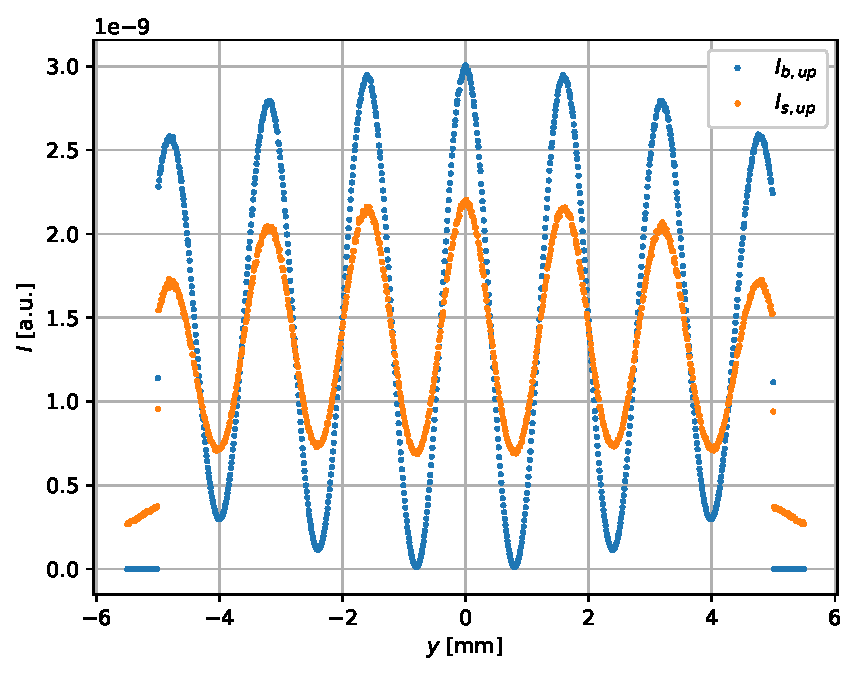
\includegraphics[width=\textwidth]{simulation-raw-intensity-up}
		\caption{$I_{b,up}$ and $I_{s,up}$.}
		\label{fig:simulation-raw-intensity-up}
	\end{subfigure}
	\hfill
	\begin{subfigure}[b]{0.45\textwidth}
		\centering
		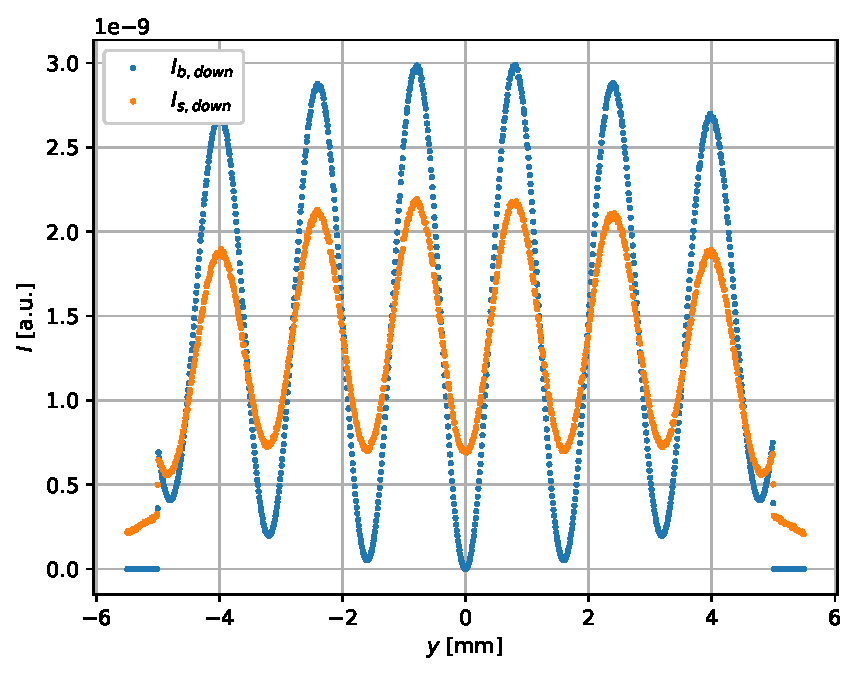
\includegraphics[width=\textwidth]{simulation-raw-intensity-down}
		\caption{$I_{b,down}$ and $I_{s,down}$.}
		\label{fig:simulation-raw-intensity-down}
	\end{subfigure}
	\centering
	\begin{subfigure}[b]{0.45\textwidth}
		\centering
		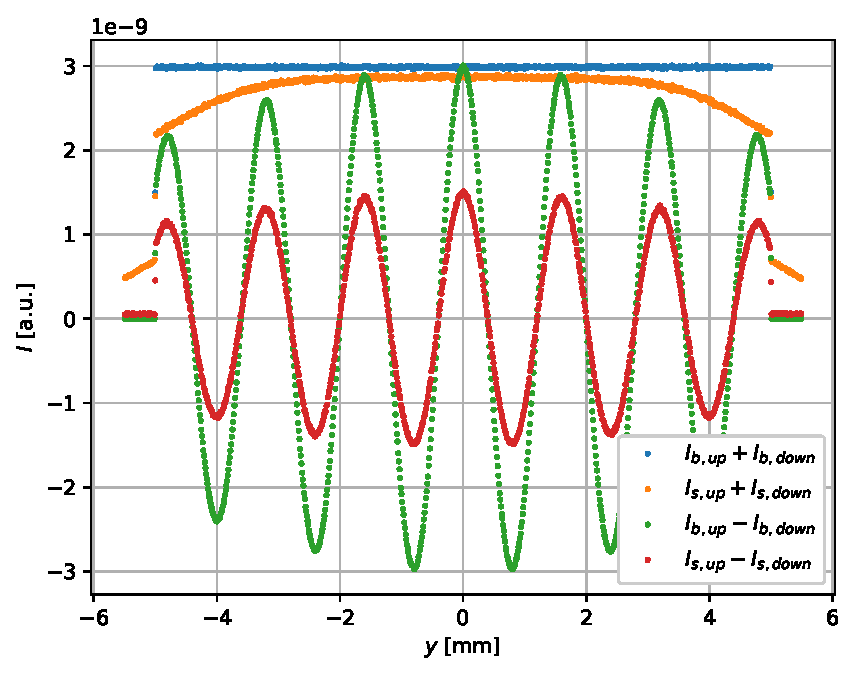
\includegraphics[width=\textwidth]{simulation-raw-intensity-differential}
		\caption{$I_{b,up} \pm I_{b,down}$ and $I_{s,up} \pm I_{s,down}$.}
		\label{fig:simulation-raw-intensity-differential}
	\end{subfigure}
	\hfill
	\begin{subfigure}[b]{0.45\textwidth}
		\centering
		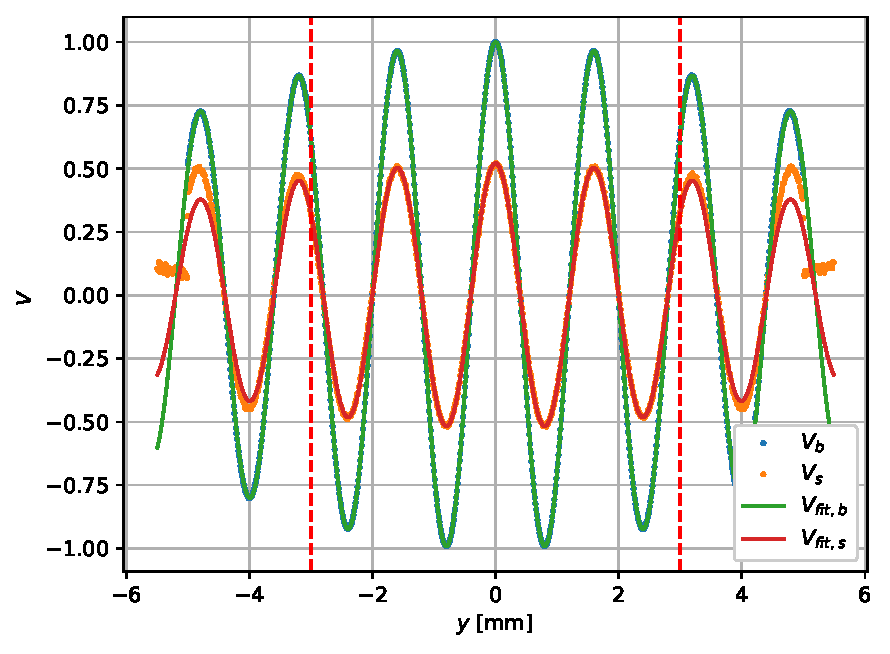
\includegraphics[width=\textwidth]{simulation-raw-intensity-pol}
		\caption{$V_b, V_s$ and fitted Gaussian modulations $V_{fit,b}, V_{fit,s}$.}
		\label{fig:simulation-raw-intensity-pol}
	\end{subfigure}
	\caption{An illustration of the detector intensity patterns recorded during simulations and how they are processed to a fit. The data corresponds to a simulated measurement using WP 8 of the $R = \SI{300}{\nano\meter}$ sample with $B_1 = \SI{5.4}{\milli\tesla}, B_2 = \SI{10.8}{\milli\tesla}$, corresponding to $\delta = \SI{900}{\nano\meter}$. The fit values are shown in Figure \ref{fig:simulation-plot-gauss-WSP-8} and \ref{fig:simulation-plot-rms-WSP-8}. Figure \ref{fig:simulation-raw-intensity-up}, \ref{fig:simulation-raw-intensity-down} show the detector intensities overlaid with and without sample for both analyzer settings (up and down). From these, signals are derived by adding and subtracting the up and down intensities. Finally, $V(y)$ is computed and from the $V(y)$ values in the middle $\SI{6}{\milli\meter}$ of the detector $P_{exp}(\delta)$ is computed by fitting modulation patterns with a Gaussian envelope or by computing the RMS.}
	\label{fig:simulation-raw-intensity}
\end{figure}

\begin{figure}[p]
	\centering
	\begin{subfigure}[b]{0.45\textwidth}
		\centering
		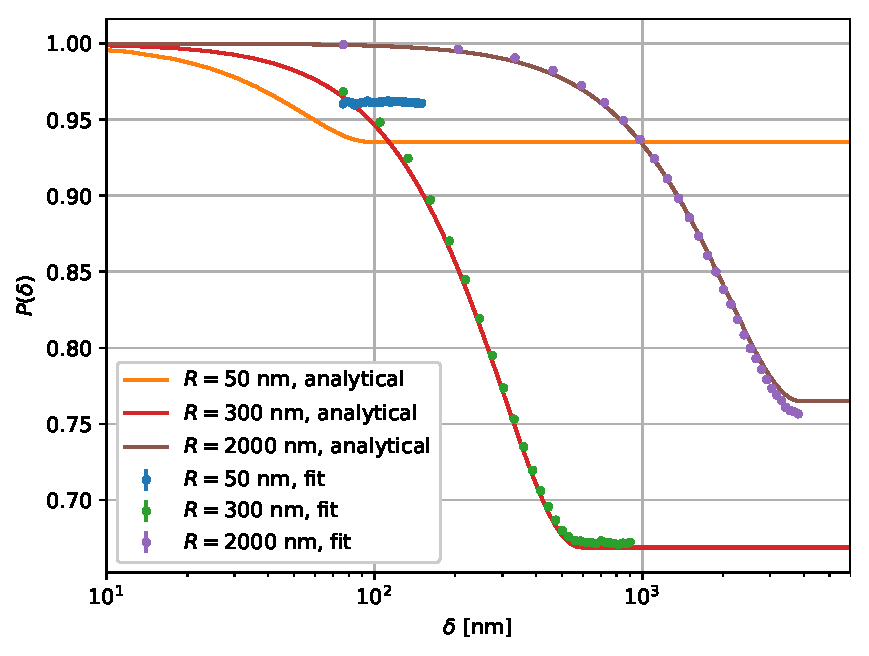
\includegraphics[width=\textwidth]{simulation-plot-gauss-FOIL-4.321}
		\caption{FOIL 4.321.}
		\label{fig:simulation-plot-gauss-FOIL-4.321}
	\end{subfigure}
	\hfill
	\begin{subfigure}[b]{0.45\textwidth}
		\centering
		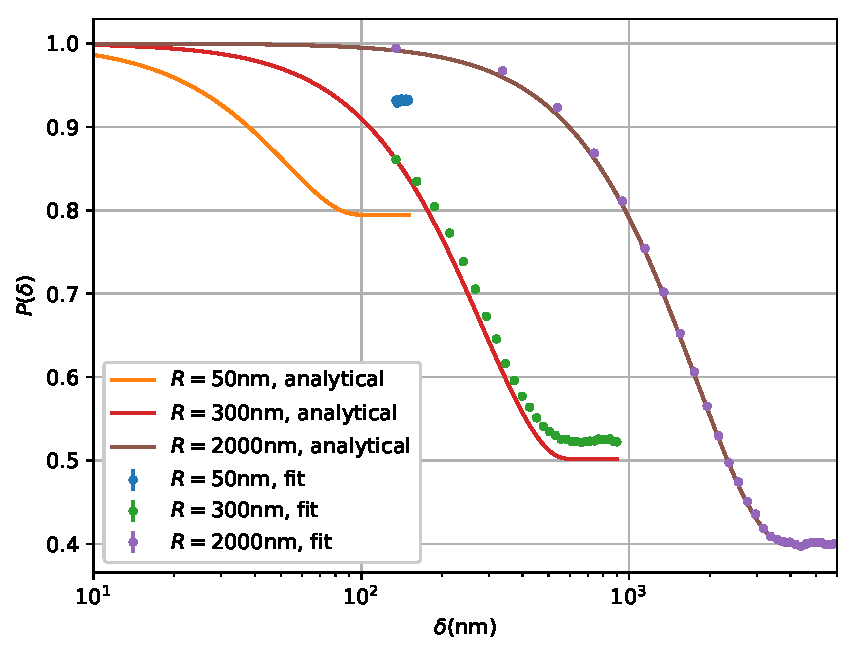
\includegraphics[width=\textwidth]{simulation-plot-gauss-FOIL-8}
		\caption{FOIL 8.}
		\label{fig:simulation-plot-gauss-FOIL-8}
	\end{subfigure}
	\centering
	\begin{subfigure}[b]{0.45\textwidth}
		\centering
		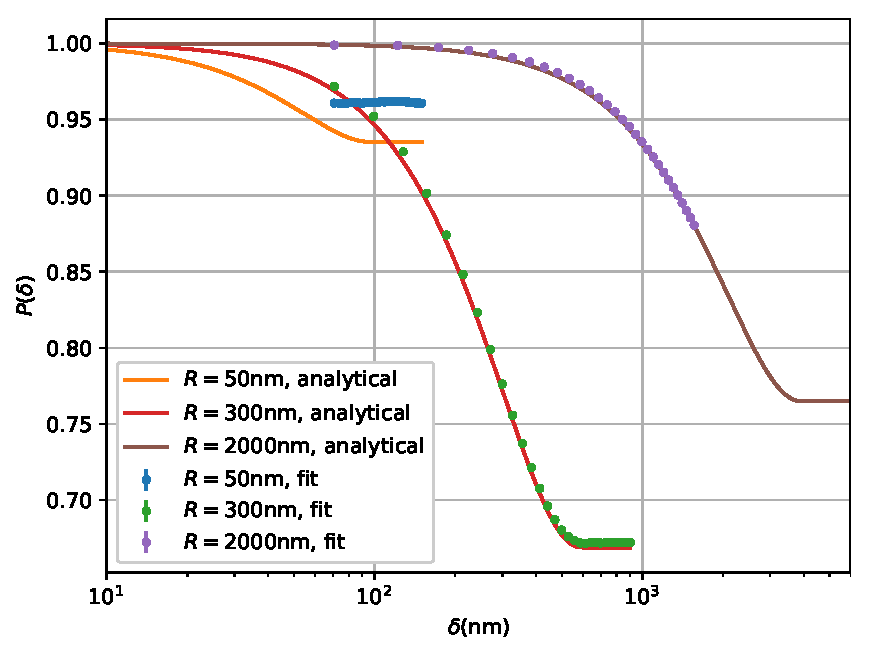
\includegraphics[width=\textwidth]{simulation-plot-gauss-WSP-4.321}
		\caption{WP 4.321.}
		\label{fig:simulation-plot-gauss-WSP-4.321}
	\end{subfigure}
	\hfill
	\begin{subfigure}[b]{0.45\textwidth}
		\centering
		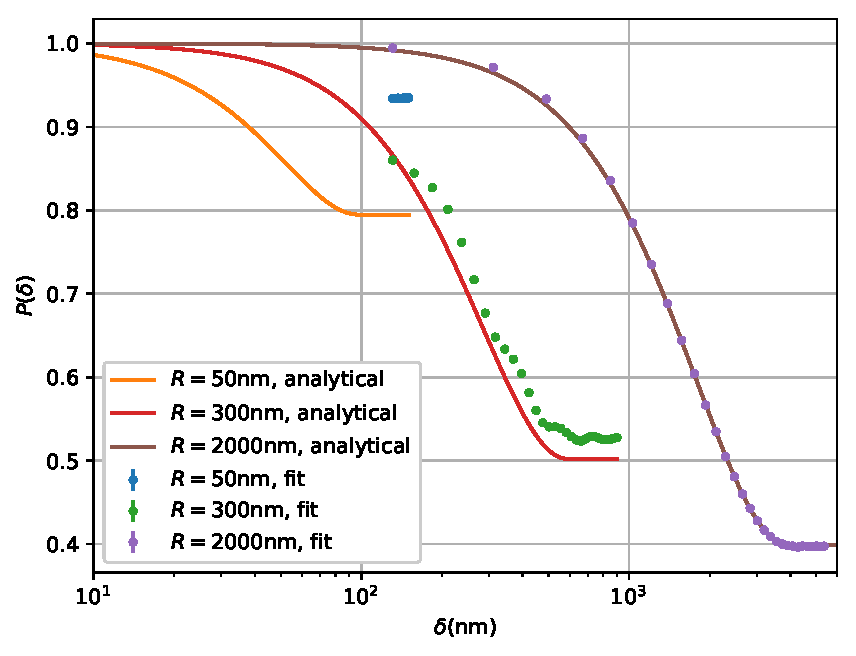
\includegraphics[width=\textwidth]{simulation-plot-gauss-WSP-8}
		\caption{WP 8.}
		\label{fig:simulation-plot-gauss-WSP-8}
	\end{subfigure}
	\centering
	\begin{subfigure}[b]{0.45\textwidth}
		\centering
		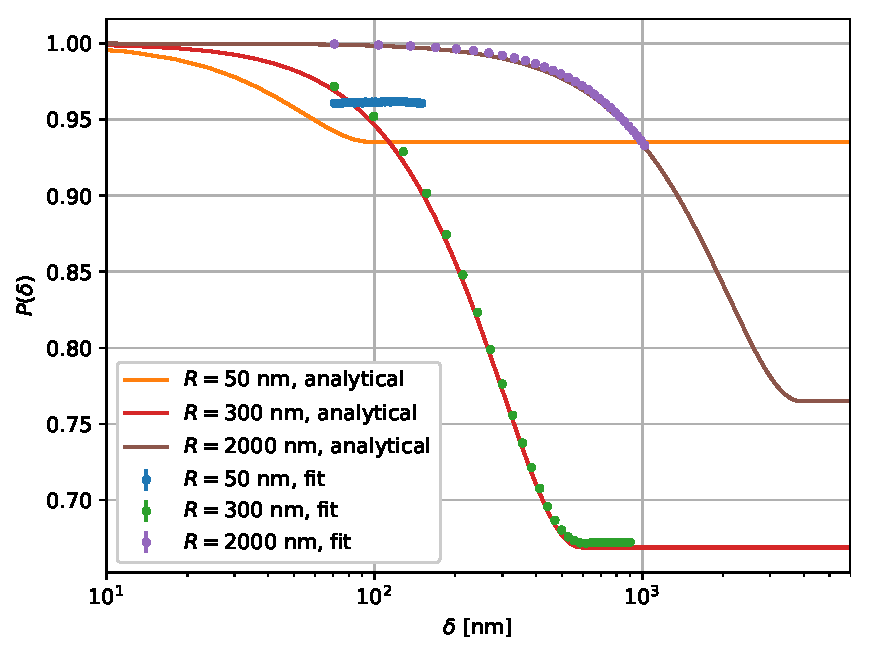
\includegraphics[width=\textwidth]{simulation-plot-gauss-ISO-4.321}
		\caption{ISO 4.321.}
		\label{fig:simulation-plot-gauss-ISO-4.321}
	\end{subfigure}
	\hfill
	\begin{subfigure}[b]{0.45\textwidth}
		\centering
		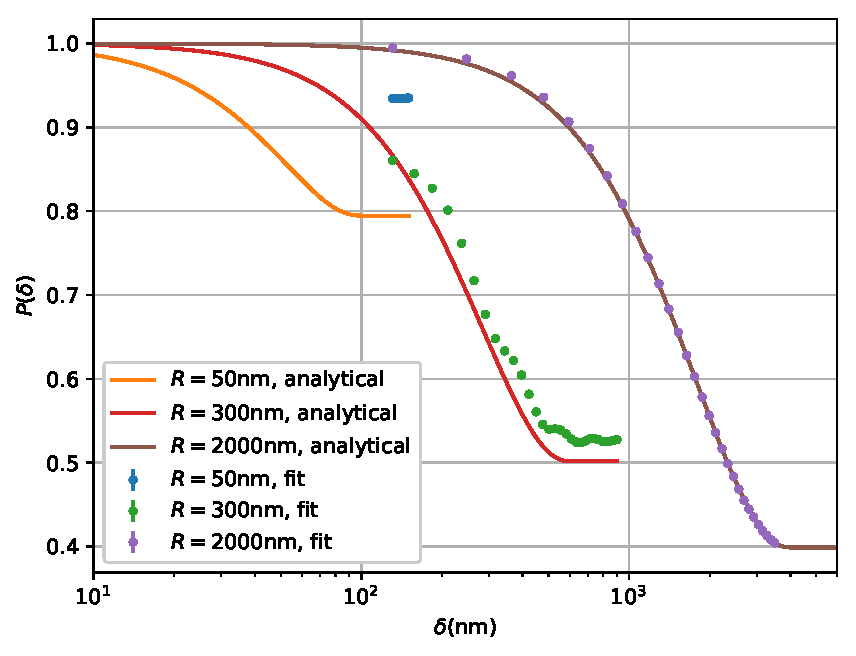
\includegraphics[width=\textwidth]{simulation-plot-gauss-ISO-8}
		\caption{ISO 8.}
		\label{fig:simulation-plot-gauss-ISO-8}
	\end{subfigure}
	\caption{$P_{exp}(\delta)$ values derived from a fit of a Gaussian modulation envelope to detector intensity simulation data. Measurements using each of the six instruments were simulated using three samples as specified in Table \ref{tab:sample-thickness} together with the corresponding analytical $P(\delta)$. The error bars are too small to be seen.}
	\label{fig:simulation-plot-gauss}
\end{figure}

\begin{figure}[p]
	\centering
	\begin{subfigure}[b]{0.45\textwidth}
		\centering
		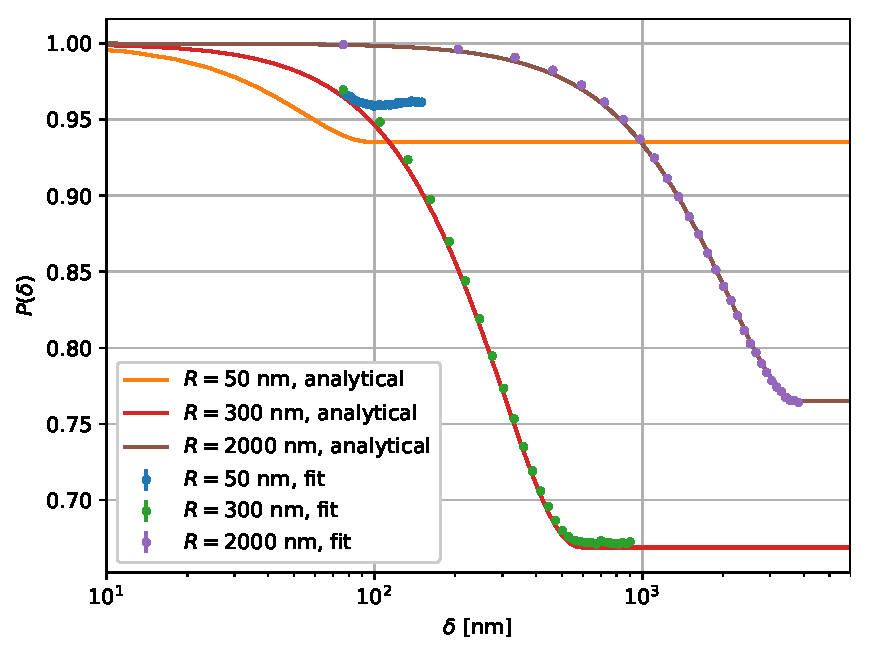
\includegraphics[width=\textwidth]{simulation-plot-rms-FOIL-4.321}
		\caption{FOIL 4.321.}
		\label{fig:simulation-plot-rms-FOIL-4.321}
	\end{subfigure}
	\hfill
	\begin{subfigure}[b]{0.45\textwidth}
		\centering
		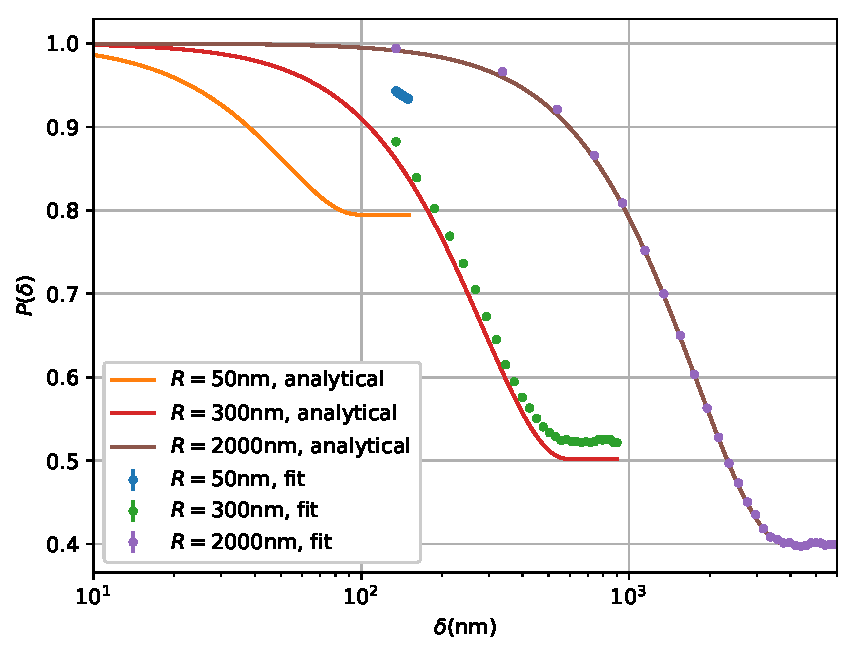
\includegraphics[width=\textwidth]{simulation-plot-rms-FOIL-8}
		\caption{FOIL 8.}
		\label{fig:simulation-plot-rms-FOIL-8}
	\end{subfigure}
	\centering
	\begin{subfigure}[b]{0.45\textwidth}
		\centering
		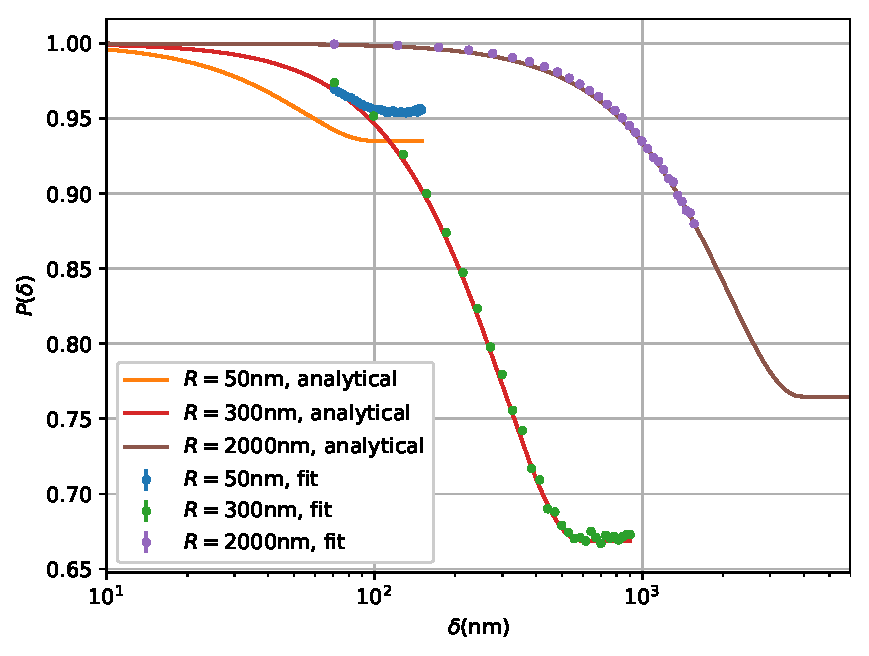
\includegraphics[width=\textwidth]{simulation-plot-rms-WSP-4.321}
		\caption{WP 4.321.}
		\label{fig:simulation-plot-rms-WSP-4.321}
	\end{subfigure}
	\hfill
	\begin{subfigure}[b]{0.45\textwidth}
		\centering
		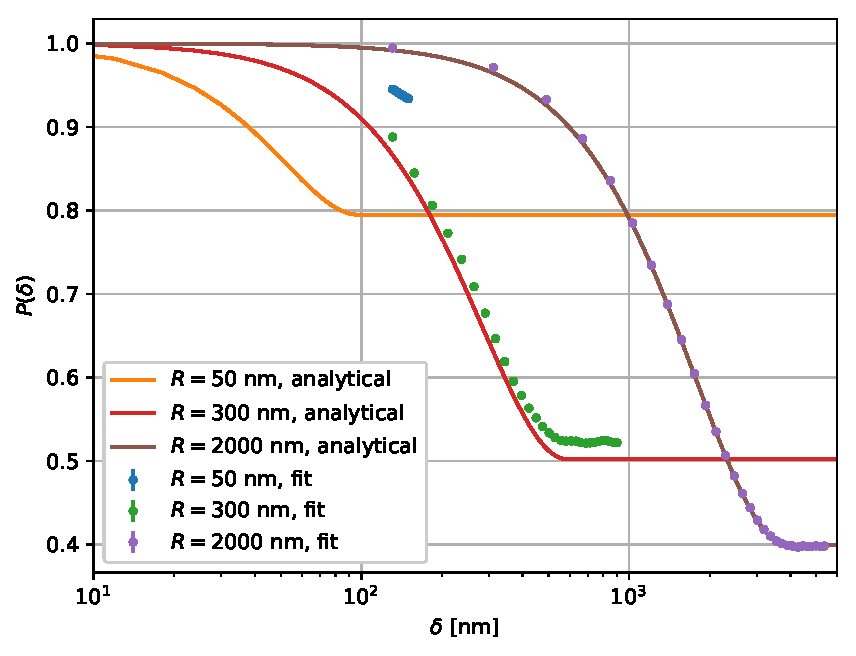
\includegraphics[width=\textwidth]{simulation-plot-rms-WSP-8}
		\caption{WP 8.}
		\label{fig:simulation-plot-rms-WSP-8}
	\end{subfigure}
	\centering
	\begin{subfigure}[b]{0.45\textwidth}
		\centering
		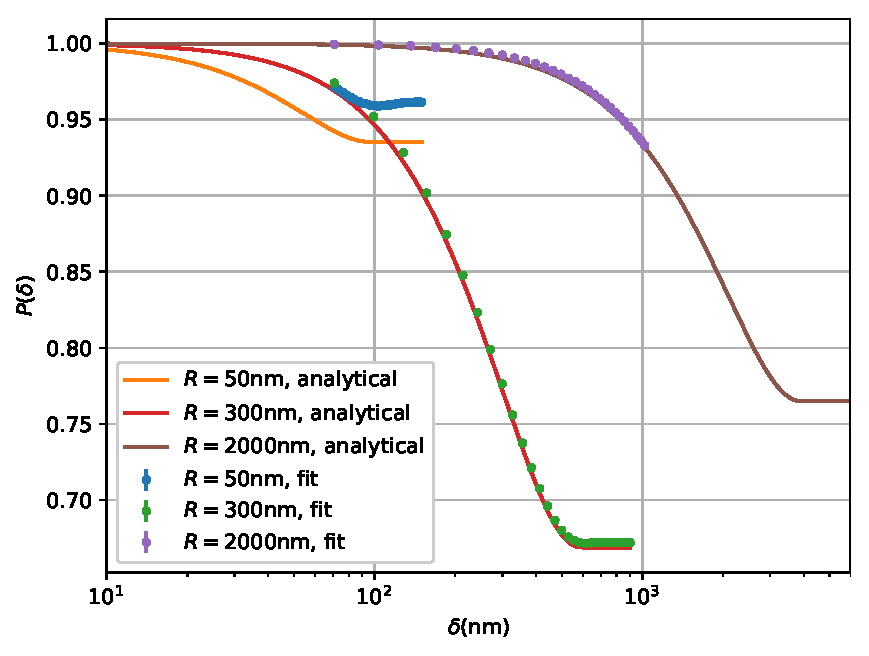
\includegraphics[width=\textwidth]{simulation-plot-rms-ISO-4.321}
		\caption{ISO 4.321.}
		\label{fig:simulation-plot-rms-ISO-4.321}
	\end{subfigure}
	\hfill
	\begin{subfigure}[b]{0.45\textwidth}
		\centering
		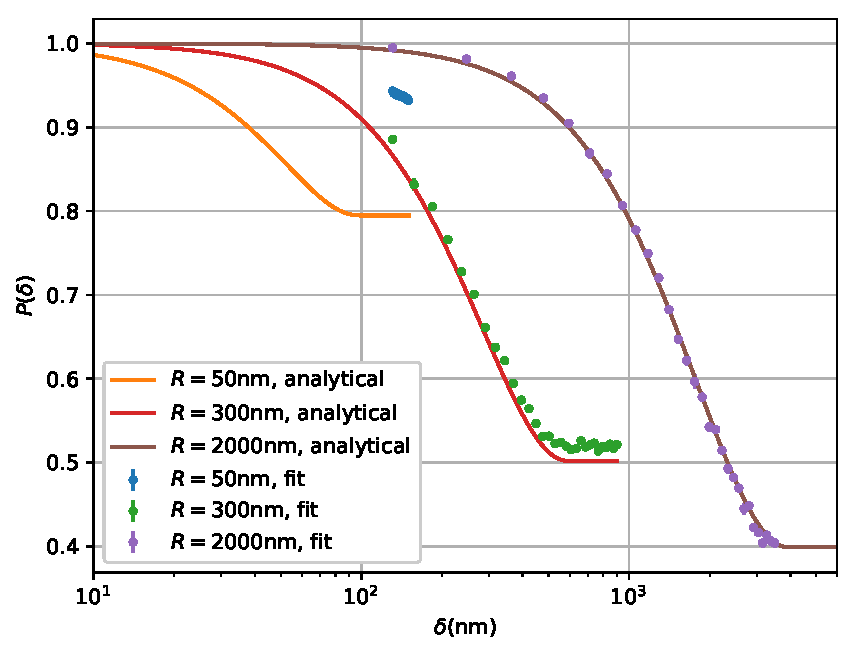
\includegraphics[width=\textwidth]{simulation-plot-rms-ISO-8}
		\caption{ISO 8.}
		\label{fig:simulation-plot-rms-ISO-8}
	\end{subfigure}
	\caption{$P_{exp}(\delta)$ values derived using the RMS method together with analytical $P(\delta)$ curves for three different samples. The data is the same as shown in Figure \ref{fig:simulation-plot-gauss}.}
	\label{fig:simulation-plot-rms}
\end{figure}

\section{Discussion}
When comparing Figures \ref{fig:simulation-plot-gauss}, \ref{fig:simulation-plot-rms}, generally speaking both analysis methods give similar results. The RMS method seems to be more consistent, better matching $P(\delta)$ for $R=\SI{2}{\micro\meter}$ in Figure \ref{fig:simulation-plot-rms-FOIL-4.321} as compared to \ref{fig:simulation-plot-gauss-FOIL-4.321}, with the Gaussian fit making an error there. The loss of polarization for $\lambda$ other than $\lambda_0$ in the foil flippers \cite{kraan2003} could perhaps explain this error, as this causes the modulation spectrum to differ from what is expected. Using RMS also gives a more reasonable fit of the $R=\SI{50}{\nano\meter}$ sample by appearing to capture some of the curvature of $P(\delta)$ in Figures \ref{fig:simulation-plot-rms-FOIL-4.321}, \ref{fig:simulation-plot-rms-WSP-4.321}, \ref{fig:simulation-plot-rms-ISO-4.321}. Although corrections compensating for a too-low detector $Q$-range \cite{kusmin2017} were not performed, it could be that the corrected analytical $P(\delta)$ curve for this sample looks somewhat like the $P_{exp}(\delta)$ fitted to data. Both methods also give a $P_{exp}(\delta)$ for $R = \SI{300}{\nano\meter}$ that is shifted upwards compared to the expected $P(\delta)$ for all instruments with $\lambda_0 = \SI{8}{\angstrom}$, indicating that $P_{exp}(\delta)$ probably accurately describes the fitted $y$-range of $V(y)$ data but cannot simply be said to estimate $P(\delta)$. Fitting only the middle $\SI{2}{\milli\meter}$ instead of the middle $\SI{6}{\milli\meter}$ of the detector reduces this error somewhat but not entirely. This can perhaps be explained by the relatively high $\tau = 0.6893$ as listed in Table \ref{tab:sample-thickness}, causing a relatively high degree of multiple scattering and a larger fraction of scattered neutrons to go undetected making $P_{exp}(\delta)$ a poor estimate of $P(\delta)$. Another reason could be the greater $\Delta\lambda$ of designs at $\lambda_0 = \SI{8}{\angstrom}$, causing errors of the type discussed in Section \ref{c3.6}. Additionally, the greater spread in scattering angles could play a role as $Q\propto 1/\lambda$, making the same $Q$ scatter into larger angles for the colder $\lambda$ values in the spectrum. This would also reduce the quality of estimate $P_{exp}(\delta)$ and the effective $Q$-range of the instrument.

This could mean that instruments with $\Delta\lambda/\lambda_0 = 0.1$ or similar like the three presented here with $\lambda_0 = \SI{8}{\angstrom}$ are more restricted for lower values of $\delta$ than predicted using the constraint model presented in Chapter \ref{c4:constraints}, meaning that measuring wide $\delta$ ranges might be harder when using colder wavelengths available at a $T=\SI{20}{\kelvin}$ using a velocity selector. 

An alternative explanation would be that $P(\delta)$ should be corrected for the spread in $\lambda$ as discussed in Section \ref{c3.6}. This would also explain why the monochromatic $P(\delta)$ expression describes the fitted $P_{exp}(\delta)$ values well when $\Delta\lambda/\lambda_0 = 0.01$ but not when $\Delta\lambda/\lambda_0 = 0.1$. It is not clear what such a correction would look like. An alternative would be to use Fourier methods, but as indicated in Section \ref{c3.6} this can be complicated by frequency resolution constraints.
%\input{mainmatter/chapter-2}
%\input{mainmatter/chapter-3}
%\input{mainmatter/chapter-4} % Create file to add

\chapter{Conclusion}
\label{chapter:conclusion}
\label{c7:conclusion}
In this work, the possibility of realizing a SEMSANS instrument at the new cold source at the Hoger Onderwijs Reactor at the Reactor Institute in Delft was explored through a combination of mathematical analysis, constrained optimization, and Monte Carlo simulations. After providing an overview of relevant theory and introducing a simplified instrument model, six combinations of three precession device options and two monochromator types with compatible wavelengths $\lambda_0$ were presented. These were analyzed in detail and measurements of known samples were simulated using the raytracing software package McStas \cite{willendrup2020}. 

The goal was to explore possibilities for an instrument that could be used to measure processes in the range of $\SI{10}{\nano\meter}$ to $\SI{5}{\micro\meter}$. It was shown by optimizing all available free parameters that when considering a beam that has an effective height $h_e$ of $\SI{10}{\milli\meter}$ on the detector in an instrument no more than about $\SI{5}{\meter}$ in length, it is impossible to measure this full range keeping the distance from sample to detector $L_s$ constant and compatible with a small-angle approximation. The precession device characteristics (field strength limitations and field interface angles) and  $h_e$ were identified as limiting factors in this initial setting using a constraint model. It was shown that by increasing the effective height to $h_e = \SI{30}{\milli\meter}$ or by using improved ferromagnetic foil flippers with a maximal field strength of $B_{max} = \SI{150}{\milli\tesla}$ instead of $\SI{30}{\milli\tesla}$, ranges such as $\SI{40}{\nano\meter}$ to $\SI{5}{\micro\meter}$ or $\SI{30}{\nano\meter}$ to $\SI{5}{\micro\meter}$ become possible. Combining these two enhancements gave an optimized range of $\SI{15}{\nano\meter}$ to $\SI{5}{\micro\meter}$, almost fully covering the target range of $\SI{10}{\nano\meter}$ to $\SI{5}{\micro\meter}$.

Additionally, the effects of using a monochromator with a greater $\Delta\lambda/\lambda_0$ in terms of modulation patterns and scattered intensity were analyzed in detail and it appears from simulation results that instruments selecting very cold neutrons with wavelength $\lambda_0 = \SI{8}{\angstrom}$ using a velocity selector might be harder to realize than instruments using a more selective pyrolytic graphite monochromator with $\lambda_0 = \SI{4.321}{\angstrom}$. This is because the relation between the measured visibility and the sample SESANS correlation function is more complex when using a broader spectrum, possibly requiring corrections to compensate for the $\lambda$-dependent interaction with the sample which were not formulated here.

In conclusion, realizing a practical SEMSANS instrument at the cold source that can measure almost the full target range might be possible. This would require sufficiently powerful precession devices and large enough beam and detector dimensions. Concrete realizations could use Wollaston prisms and a velocity selector with a colder wavelength of about $\lambda_0 = 9 - 10~\unit{\angstrom}$ or improved foil flippers with a pyrolytic graphite monochromator at a warmer wavelength of about $\lambda_0 = 3 - 4~\unit{\angstrom}$. The measurement analysis and interpretation might be easier when using the latter option with a pyrolytic graphite monochromator for the reasons indicated above.

\section{Future work}
\label{c7.1}
The purpose of this work was to give a first understanding of what is possible in terms of designing SEMSANS instruments for the cold source. For this reason, many factors were abstracted, and the instrument model used is in many ways idealized. For instance, the idealized beam has a uniform profile with slight divergence and a $\lambda$-spectrum exactly described by a Maxwell-Boltzmann spectrum at $T= \SI{20}{\kelvin}$, with an idealized monochromator selecting a Gaussian distribution of wavelengths. These and other simplifications leave work to be done in terms of more realistic analysis and simulations considering the profile and spectrum of the cold source and how the source is collimated. The same goes for simulating the physical precession devices, monochromators, and the polarizer and analyzer. Such realistic simulations would also make more accurate intensity estimates possible, which is an essential step before any potential realization of an instrument. In addition to more realistic simulations, Monte Carlo simulations of optimized designs presented in this work could be performed to learn if it is possible to measure spin-echo lengths over a range of $\SI{15}{\nano\meter}$ to $\SI{5}{\micro\meter}$. Such additional simulations were not performed due to time constraints.

Finally, more detailed studies of tolerable acceptance angles in SEMSANS as well as the effect of broader $\lambda$-spectra on measurement ranges would make it possible to optimize designs further than was done in this work and make it easier to estimate what can practically be measured using a given design. In addition to implementing the existing correction for limited acceptance angles \cite{kusmin2017}, it might be possible to correct for the broader $\lambda$-spectrum as well by computing the effect on modulation visibility or using Fourier methods, meaning that designs using velocity selectors and broader $\lambda$-spectra might not be further limited but require a different treatment than the one presented in this work.

\section{Reproducibility}
\label{c7.2}
All code used in this research is publicly available online in the form of a Github repository\footnote{\url{https://github.com/tbvanderwoude/semsans}}. It contains an overview of how McStas simulations can be reproduced using the provided instrument and component files. It also lists the requirements for running the included Python notebooks and other code. This includes an instrument model implemented in Python together with code that can compute optimal designs in the sense considered in this work.

%% Prevent urls running into margins in bibliography
\setcounter{biburlnumpenalty}{7000}
\setcounter{biburllcpenalty}{7000}
\setcounter{biburlucpenalty}{7000}

%% Add bibliography
\printbibliography[heading=bibintoc,title=References]

%% ----------------------------------------------------------------------
%%    Appendix (Letters for chapters)
%% ----------------------------------------------------------------------

\appendix

%\chapter{Source Code Example}
%\label{chapter:title}

\emph{Adding source code to your report/thesis is supported with the package {\normalfont\texttt{listings}}. An example can be found below. Files can be added using {\normalfont\texttt{\textbackslash lstinputlisting[language=<language>]\{<filename>\}}}.}

\begin{lstlisting}[language=Python]
"""
ISA Calculator: import the function, specify the height and it will return a
list in the following format: [Temperature,Density,Pressure,Speed of Sound].
Note that there is no check to see if the maximum altitude is reached.
"""

import math
g0 = 9.80665
R = 287.0
layer1 = [0, 288.15, 101325.0]
alt = [0,11000,20000,32000,47000,51000,71000,86000]
a = [-.0065,0,.0010,.0028,0,-.0028,-.0020]

def atmosphere(h):
    for i in range(0,len(alt)-1):
        if h >= alt[i]:
            layer0 = layer1[:]
            layer1[0] = min(h,alt[i+1])
            if a[i] != 0:
                layer1[1] = layer0[1] + a[i]*(layer1[0]-layer0[0])
                layer1[2] = layer0[2] * (layer1[1]/layer0[1])**(-g0/(a[i]*R))
            else:
                layer1[2] = layer0[2]*math.exp((-g0/(R*layer1[1]))*(layer1[0]-layer0[0]))
    return [layer1[1],layer1[2]/(R*layer1[1]),layer1[2],math.sqrt(1.4*R*layer1[1])]
\end{lstlisting}

%\input{appendix/appendix-b}
%\input{appendix/appendix-c} % Create file to add

\end{document}
